% =====================================================================
%  Chapter 20: Capstone Projects and Extended Explorations
%  Sections 20.1 and 20.2
% =====================================================================

\chapter{Capstone Projects and Extended Explorations}
\label{ch:20}

Chapter \ref{ch:19} closed the main story.  We began the book with points and
vectors, and we ended with fields, flux, conservation laws, and the generalized Stokes
theorem.  The path was long, but the pattern became simple:

\[
    \text{local change}
    \quad\longleftrightarrow\quad
    \text{derivatives}
    \quad\longleftrightarrow\quad
    \text{boundary measurements}
    \quad\longleftrightarrow\quad
    \text{global behavior}.
\]

This last chapter is a workshop.  The projects are meant to make the ideas visible,
computable, and explainable.  Some can be done by hand.  Some are better with
graphing software.  Some are short reports.  A good project should not only get an
answer; it should tell a mathematical story.

\section{Geometry and visualization projects}
\label{sec:20.1}

Geometry was the first language of the book.  Before derivatives, integrals, and forms,
we needed points, vectors, curves, surfaces, and coordinates.  These projects return to
that beginning, but now with the whole course available.

The goal is not to make pretty pictures only.  A picture should answer a question:
Where does the surface bend?  Where does a parametrization collapse?  Which direction
is normal?  What does a linear approximation really approximate?

\subsection{Project 1: build and classify quadric surfaces}

A quadric surface is described by a second-degree equation in \(x,y,z\).  In Section
\ref{sec:4.4}, we learned the main trick:

\[
\boxed{
    \text{To understand a quadric surface, slice it.}
}
\]

A surface that looks mysterious in three dimensions often becomes clear when we set
one variable equal to a constant and study the resulting trace.

\subsubsection*{A seed example: a shifted ellipsoid}

Consider
\[
    \frac{(x-1)^2}{9}+\frac{y^2}{4}+(z+2)^2=1.
\]
The shifted terms tell us the center:
\[
    (1,0,-2).
\]
The denominators tell us the axis lengths:
\[
    3 \text{ in the }x\text{-direction},\qquad
    2 \text{ in the }y\text{-direction},\qquad
    1 \text{ in the }z\text{-direction}.
\]
So the surface is an ellipsoid, stretched most in the \(x\)-direction and least in the
\(z\)-direction.

A few slices confirm this.

If \(z=-2\), then
\[
    \frac{(x-1)^2}{9}+\frac{y^2}{4}=1,
\]
an ellipse in the horizontal plane through the center.

If \(y=0\), then
\[
    \frac{(x-1)^2}{9}+(z+2)^2=1,
\]
an ellipse in the \(xz\)-plane.

If \(x=1\), then
\[
    \frac{y^2}{4}+(z+2)^2=1,
\]
an ellipse in the \(yz\)-plane.

The surface was not guessed from a memorized shape.  It was read from its slices.

\begin{figure}[h]
\centering
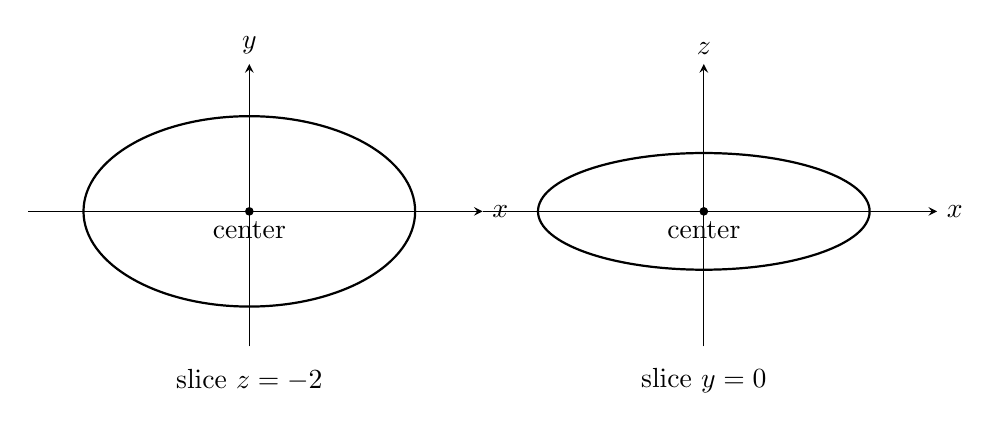
\begin{tikzpicture}[scale=0.78, >=stealth]
    \begin{scope}
        \draw[->] (-3.6,0) -- (3.8,0) node[right] {\(x\)};
        \draw[->] (0,-2.2) -- (0,2.4) node[above] {\(y\)};
        \draw[thick] (0,0) ellipse (2.7 and 1.55);
        \fill (0,0) circle (2pt);
        \node[below] at (0,0) {center};
        \node at (0,-2.75) {slice \(z=-2\)};
    \end{scope}

    \begin{scope}[shift={(7.4,0)}]
        \draw[->] (-3.6,0) -- (3.8,0) node[right] {\(x\)};
        \draw[->] (0,-2.2) -- (0,2.4) node[above] {\(z\)};
        \draw[thick] (0,0) ellipse (2.7 and 0.95);
        \fill (0,0) circle (2pt);
        \node[below] at (0,0) {center};
        \node at (0,-2.75) {slice \(y=0\)};
    \end{scope}
\end{tikzpicture}
\caption{Two traces of the same ellipsoid.  The traces reveal the stretches.}
\end{figure}

\subsubsection*{Your task}

Create a visual gallery of at least six quadric surfaces.

Use six or more of the following:

\[
\begin{array}{c}
x^2+y^2=4,\\[1mm]
y=x^2,\\[1mm]
z=x^2+y^2,\\[1mm]
z=x^2-y^2,\\[1mm]
\dfrac{x^2}{9}+\dfrac{y^2}{4}+z^2=1,\\[4mm]
x^2+y^2-z^2=1,\\[1mm]
z^2-x^2-y^2=1,\\[1mm]
z^2=x^2+y^2,\\[1mm]
\dfrac{(x-1)^2}{4}+\dfrac{(y+2)^2}{9}+\dfrac{z^2}{16}=1.
\end{array}
\]

For each surface, include:

\[
\begin{array}{ll}
1. & \text{the equation,}\\
2. & \text{the name of the surface,}\\
3. & \text{three traces or cross-sections,}\\
4. & \text{a hand sketch, physical model, or computer plot,}\\
5. & \text{one sentence explaining how signs, coefficients, or missing variables shape it.}
\end{array}
\]

\subsubsection*{Questions to answer}

\begin{enumerate}
\item Which surfaces are connected?  Which have two separate pieces?

\item Which equations contain a missing variable?  What geometric effect does that
missing variable have?

\item Which surfaces have horizontal traces that are circles?  Which have horizontal
traces that are ellipses?  Which have hyperbolas?

\item What changes when
\[
    x^2+y^2-z^2=1
\]
is replaced by
\[
    z^2-x^2-y^2=1?
\]

\item What changes when an equation is shifted, as in
\[
    \frac{(x-1)^2}{4}+\frac{(y+2)^2}{9}+\frac{z^2}{16}=1?
\]
\end{enumerate}

\subsubsection*{What to hand in}

Write a short illustrated report.  It should include a table like this:

\[
\begin{array}{c|c|c|c}
\text{Equation} & \text{Name} & \text{Useful traces} & \text{Geometry note} \\ \hline
z=x^2+y^2 & \text{elliptic paraboloid} &
z=c & \text{horizontal ellipses grow upward}\\[1mm]
z=x^2-y^2 & \text{hyperbolic paraboloid} &
x=0,\ y=0 & \text{one slice bends up, one bends down}
\end{array}
\]

A good gallery should make a reader feel that a quadric equation is not a code to
memorize.  It is a set of instructions for building a shape.

\subsection{Project 2: visualize tangent planes and linear approximations}

Chapter \ref{ch:7} gave the tangent plane formula for a differentiable graph
\[
    z=f(x,y).
\]
At the point
\[
    (a,b,f(a,b)),
\]
the tangent plane is
\[
\boxed{
    z=f(a,b)+f_x(a,b)(x-a)+f_y(a,b)(y-b).
}
\]
This plane is the best first-order model of the surface near the point.

The word ``near'' matters.  A tangent plane is not a replacement for the whole surface.
It is a local microscope.

\subsubsection*{A seed example: a curved roof}

Suppose a small roof has height
\[
    f(x,y)=5+\frac12x-\frac14y+\frac18x^2-\frac1{16}y^2+\frac18xy.
\]
At
\[
    (a,b)=(2,1),
\]
the height is
\[
\begin{aligned}
    f(2,1)
    &=
    5+1-\frac14+\frac12-\frac1{16}+\frac14\\
    &=
    \frac{103}{16}.
\end{aligned}
\]
The partial derivatives are
\[
    f_x(x,y)=\frac12+\frac14x+\frac18y,
\]
and
\[
    f_y(x,y)=-\frac14-\frac18y+\frac18x.
\]
So
\[
    f_x(2,1)=\frac98,
    \qquad
    f_y(2,1)=-\frac18.
\]
The tangent plane is
\[
\boxed{
    z=\frac{103}{16}+\frac98(x-2)-\frac18(y-1).
}
\]

Now compare the true height with the plane at a nearby point, say
\[
    (2.2,0.9).
\]
The tangent plane predicts
\[
    L(2.2,0.9)
    =
    \frac{103}{16}
    +
    \frac98(0.2)
    -
    \frac18(-0.1).
\]
The actual error is
\[
    f(2.2,0.9)-L(2.2,0.9).
\]
If we move the point twice as close to \((2,1)\), the error should become much smaller.
That is what differentiability means: the linear model wins at small scales.

\begin{figure}[h]
\centering
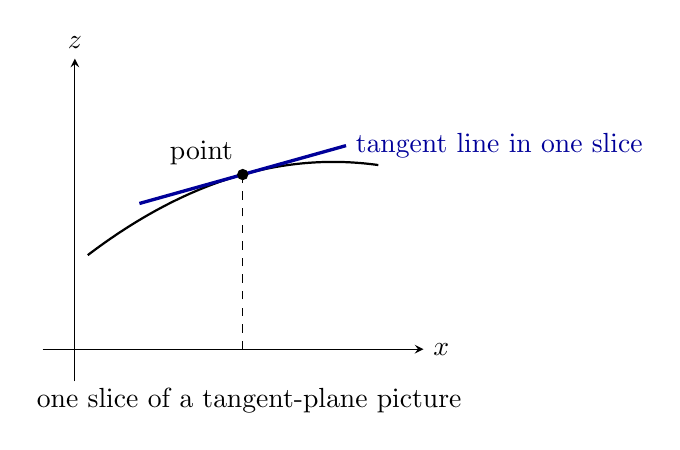
\begin{tikzpicture}[scale=0.82, >=stealth]
    \draw[->] (-0.5,0) -- (5.4,0) node[right] {\(x\)};
    \draw[->] (0,-0.5) -- (0,4.5) node[above] {\(z\)};

    \draw[thick, domain=0.2:4.7, samples=80, smooth, variable=\x]
        plot ({\x},{1.3+0.8*\x-0.10*\x*\x});

    % Corrected tangent line based on z = 0.28x + 1.976
    \draw[blue!60!black, very thick] (1.0,2.256) -- (4.2,3.152);
    \node[blue!60!black, right] at (4.2,3.152) {tangent line in one slice};

    % Corrected point coordinates
    \fill (2.6,2.704) circle (2.5pt);
    \node[above left] at (2.6,2.704) {point};

    % Corrected dashed line height
    \draw[dashed] (2.6,0) -- (2.6,2.704);
    \node at (2.7,-0.8) {one slice of a tangent-plane picture};
\end{tikzpicture}
\caption{A tangent plane is seen in every slice as a tangent line.}
\end{figure}

\subsubsection*{Your task}

Choose one smooth surface and one nonsmooth surface.

For the smooth surface, use one of these or choose your own:

\[
\begin{array}{c}
f_1(x,y)=4+x-\frac12y-\frac14x^2-\frac18y^2,\\[1mm]
f_2(x,y)=5+\frac12x-\frac14y+\frac18x^2-\frac1{16}y^2+\frac18xy,\\[1mm]
f_3(x,y)=\sin x\cos y.
\end{array}
\]

For the nonsmooth surface, use one of these:

\[
\begin{array}{c}
g_1(x,y)=\sqrt{x^2+y^2},\\[1mm]
g_2(x,y)=|x|+|y|.
\end{array}
\]

\subsubsection*{Part A. The smooth surface}

Pick a point \((a,b)\).  Then:

\begin{enumerate}
\item Compute
\[
    f(a,b),\qquad f_x(a,b),\qquad f_y(a,b).
\]

\item Write the linear approximation
\[
\boxed{
    L(x,y)=f(a,b)+f_x(a,b)(x-a)+f_y(a,b)(y-b).
}
\]

\item Plot the surface
\[
    z=f(x,y)
\]
and the tangent plane
\[
    z=L(x,y)
\]
on the same axes.

\item Choose several nearby displacement vectors
\[
    \mathbf h=(h,k).
\]
For each one, compute the error
\[
    E(\mathbf h)=f(a+h,b+k)-L(a+h,b+k).
\]

\item Make a table containing
\[
    \|\mathbf h\|,
    \qquad
    |E(\mathbf h)|,
    \qquad
    \frac{|E(\mathbf h)|}{\|\mathbf h\|},
    \qquad
    \frac{|E(\mathbf h)|}{\|\mathbf h\|^2}.
\]
\end{enumerate}

The first ratio should get small as
\[
    \|\mathbf h\|\to0.
\]
That is the signature of differentiability.

\subsubsection*{Part B. The nonsmooth surface}

At the origin, draw or plot
\[
    z=\sqrt{x^2+y^2}
\]
or
\[
    z=|x|+|y|.
\]

Then answer:

\begin{enumerate}
\item Does the surface look like it has one tangent plane at the origin?

\item What do the slices along the \(x\)-axis and \(y\)-axis look like?

\item Why is a tangent plane not the same thing as matching a few coordinate slices?

\item How does the picture explain the warning from Chapter \ref{ch:7}: partial
information in some directions does not guarantee a true linear approximation in all
directions?
\end{enumerate}

\subsubsection*{What to hand in}

Your report should include:

\begin{enumerate}
\item the smooth surface and point you chose,

\item the tangent plane calculation,

\item one plot or hand sketch showing the surface and tangent plane together,

\item an error table,

\item one plot or hand sketch of the nonsmooth surface,

\item a paragraph explaining why the smooth surface has a local linear model and the
nonsmooth surface does not.
\end{enumerate}

The main lesson is visual: differentiability means that the graph becomes flatter and
flatter under a microscope.  A corner, cusp, or cone tip refuses to become one plane.

\subsection{Project 3: plot gradient fields and contour maps together}

A contour map shows level sets:
\[
    f(x,y)=c.
\]
A gradient field shows vectors:
\[
    \nabla f(x,y).
\]
Chapter \ref{ch:9} connected them:

\[
\boxed{
    \nabla f \text{ is perpendicular to the level curves of } f.
}
\]

This project asks you to draw both at once.

\subsubsection*{A seed example: temperature on a plate}

Let
\[
    T(x,y)=20+4x-y-x^2-\frac12y^2.
\]
Then
\[
    \nabla T(x,y)=(4-2x,\,-1-y).
\]
At the point
\[
    (1,-1),
\]
we get
\[
    \nabla T(1,-1)=(2,0).
\]
So the temperature rises fastest toward the positive \(x\)-direction.

The level curve through \((1,-1)\) has tangent directions \((u,v)\) satisfying
\[
    \nabla T(1,-1)\cdot(u,v)=0.
\]
Thus
\[
    (2,0)\cdot(u,v)=0,
\]
so
\[
    u=0.
\]
The tangent direction is vertical.  The gradient is horizontal.  They are perpendicular.

\begin{figure}[h]
\centering
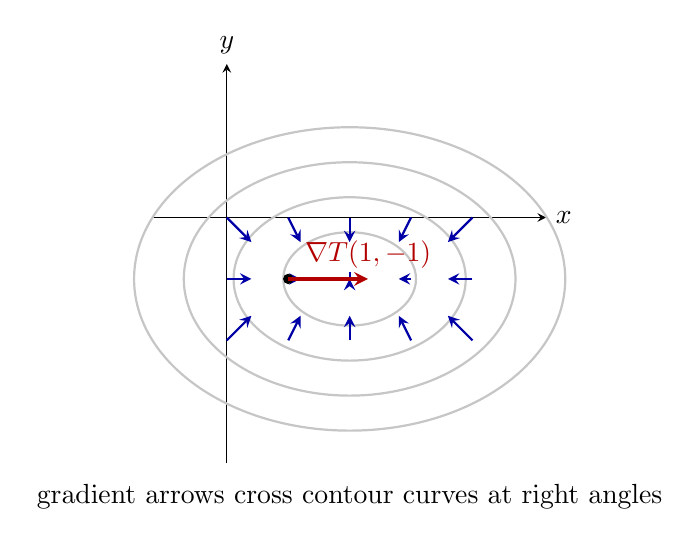
\begin{tikzpicture}[scale=0.78, >=stealth]
    \draw[->] (-1.2,0) -- (5.2,0) node[right] {\(x\)};
    \draw[->] (0,-4.0) -- (0,2.5) node[above] {\(y\)};

    \foreach \r in {0.8,1.4,2.0,2.6} {
        \draw[gray!45, thick] (2,-1) ellipse ({1.35*\r} and {0.95*\r});
    }

    % Corrected gradient field: y-component scales twice as fast as x-component
    \foreach \x/\y in {0/0,1/0,2/0,3/0,4/0,0/-1,1/-1,2/-1,3/-1,4/-1,0/-2,1/-2,2/-2,3/-2,4/-2} {
        \draw[->, blue!65!black, thick]
            (\x,\y) -- ++({0.2*(2-\x)},{0.4*(-1-\y)});
    }

    \fill (1,-1) circle (2.4pt);
    \draw[->, red!70!black, very thick] (1,-1) -- (2.3,-1)
        node[above] {\(\nabla T(1,-1)\)};

    \node at (2,-4.55) {gradient arrows cross contour curves at right angles};
\end{tikzpicture}
\caption{Contours and gradient arrows carry different information, but they fit
together geometrically.}
\end{figure}

\subsubsection*{Your task}

Choose two scalar fields from the list below:

\[
\begin{array}{c}
f_1(x,y)=4-\dfrac{x^2}{4}-y^2,\\[3mm]
f_2(x,y)=xy,\\[1mm]
f_3(x,y)=6+2x-y-\dfrac14x^2-\dfrac12y^2,\\[3mm]
f_4(x,y)=\sin x+\cos y,\\[1mm]
f_5(x,y)=\ln\sqrt{x^2+y^2}\quad\text{on }\mathbb R^2\setminus\{(0,0)\}.
\end{array}
\]

For each chosen field:

\begin{enumerate}
\item Compute
\[
    \nabla f.
\]

\item Draw several level curves
\[
    f(x,y)=c.
\]

\item Draw gradient arrows on the same picture.

\item Pick three points on three different level curves.  At each point, show that the
gradient is perpendicular to the level curve.  You may do this by using
\[
    f_x\,dx+f_y\,dy=0
\]
for tangent directions.

\item Find the critical points, if any:
\[
    \nabla f=\mathbf 0.
\]

\item Where possible, use the Hessian from Chapter \ref{ch:9} to classify the critical
points.
\end{enumerate}

\subsubsection*{Extra exploration: following the arrows}

A path
\[
    \mathbf r(t)
\]
that follows the gradient field satisfies
\[
    \mathbf r'(t)=\nabla f(\mathbf r(t)).
\]
Such a path climbs the scalar field as quickly as possible at each point.

For one of your chosen fields, sketch a few paths that follow the gradient arrows.

Then answer:

\begin{enumerate}
\item Do the paths cross level curves at right angles?

\item Do they move toward a maximum, away from a minimum, or through a saddle?

\item What happens near a critical point?

\item If your field is
\[
    f_5(x,y)=\ln\sqrt{x^2+y^2},
\]
what role does the missing origin play?
\end{enumerate}

\subsubsection*{What to hand in}

Your report should include:

\begin{enumerate}
\item two combined contour-gradient plots,

\item the gradient formulas,

\item at least three perpendicularity checks,

\item critical point calculations,

\item Hessian classifications where possible,

\item a paragraph comparing the two fields.  Which one looks like a bowl, a hill, a
saddle, a wave, or a singular field?
\end{enumerate}

The goal is to make the gradient feel less like a formula and more like a geometric
compass.

\subsection{Project 4: compare parameter grids on a sphere, torus, and cone}

A parametrization is a coordinate system on a surface.  It does more than draw the
surface.  It creates a grid, gives tangent directions, chooses an orientation, and
supplies the area scale factor
\[
    \|\mathbf r_u\times \mathbf r_v\|.
\]

Different parametrizations reveal different parts of the geometry.  They also hide
different parts.

\subsubsection*{The three surfaces}

Use the following parametrizations.

\subsubsection*{1. Sphere of radius \(a\)}

\[
    \mathbf r_S(\theta,\phi)
    =
    (a\sin\phi\cos\theta,\,
     a\sin\phi\sin\theta,\,
     a\cos\phi),
\]
where
\[
    0\le\theta\le2\pi,
    \qquad
    0\le\phi\le\pi.
\]

\subsubsection*{2. Torus}

Let \(R>r>0\).  The torus with major radius \(R\) and minor radius \(r\) is
\[
    \mathbf r_T(\theta,\phi)
    =
    \bigl((R+r\cos\phi)\cos\theta,\,
          (R+r\cos\phi)\sin\theta,\,
          r\sin\phi\bigr),
\]
where
\[
    0\le\theta\le2\pi,
    \qquad
    0\le\phi\le2\pi.
\]

\subsubsection*{3. Upper cone}

\[
    \mathbf r_C(\theta,s)
    =
    (s\cos\theta,\,
     s\sin\theta,\,
     s),
\]
where
\[
    0\le\theta\le2\pi,
    \qquad
    0\le s\le a.
\]

\begin{figure}[h]
\centering
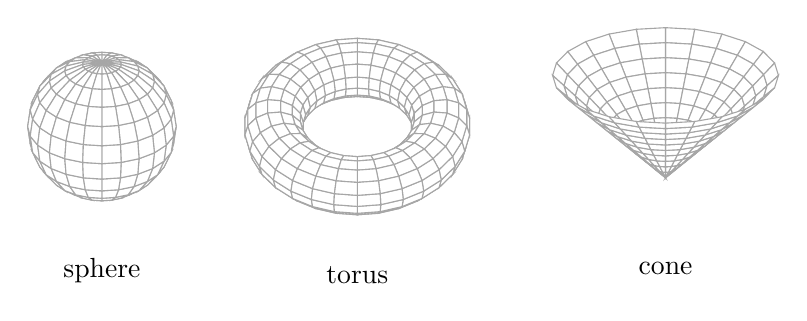
\begin{tikzpicture}
    % --- Sphere ---
    \begin{axis}[
        name=sphere,
        width=5.5cm, height=5.5cm,
        view={30}{30},
        axis equal image,
        axis lines=none,
    ]
        \addplot3[
            surf,
            fill=white,
            faceted color=gray!70,
            z buffer=sort,
            samples=25,
            samples y=13,
            domain=0:360,
            y domain=0:180
        ]
        ({sin(y)*cos(x)}, {sin(y)*sin(x)}, {cos(y)});
    \end{axis}
    \node at (sphere.south) [yshift=-2mm] {sphere};

    % --- Torus ---
    \begin{axis}[
        name=torus,
        at={(sphere.east)}, anchor=west,
        width=5.5cm, height=5.5cm,
        view={30}{45},
        axis equal image,
        axis lines=none,
    ]
        \addplot3[
            surf,
            fill=white,
            faceted color=gray!70,
            z buffer=sort,
            samples=31,
            samples y=15,
            domain=0:360,
            y domain=0:360
        ]
        ({(2+0.7*cos(y))*cos(x)}, {(2+0.7*cos(y))*sin(x)}, {0.7*sin(y)});
    \end{axis}
    \node at (torus.south) [yshift=-2mm] {torus};

    % --- Upper Cone ---
    \begin{axis}[
        name=cone,
        at={(torus.east)}, anchor=west,
        width=5.5cm, height=5.5cm,
        view={30}{25},
        axis equal image,
        axis lines=none,
    ]
        \addplot3[
            surf,
            fill=white,
            faceted color=gray!70,
            z buffer=sort,
            samples=25,
            samples y=11,
            domain=0:360,
            y domain=0:2.5
        ]
        ({y*cos(x)}, {y*sin(x)}, {y});
    \end{axis}
    \node at (cone.south) [yshift=-2mm] {cone};

\end{tikzpicture}
\caption{The same two-parameter idea produces very different surface grids.}
\end{figure}

\subsubsection*{Your task}

For each surface:

\begin{enumerate}
\item Draw the parameter domain.

\item Draw the two families of parameter curves:
\[
    \theta=\text{constant},
    \qquad
    \phi=\text{constant}
\]
or
\[
    \theta=\text{constant},
    \qquad
    s=\text{constant}.
\]

\item Compute the two tangent vectors.

\item Compute the magnitude of the cross product:
\[
    \|\mathbf r_u\times\mathbf r_v\|.
\]

\item Find where the parametrization repeats points.

\item Find where the parametrization collapses or becomes nonregular:
\[
    \mathbf r_u\times\mathbf r_v=\mathbf 0.
\]

\item Describe how the parameter grid stretches or crowds on the surface.
\end{enumerate}

\subsubsection*{Useful checkpoints}

For the sphere,
\[
\boxed{
    \|\mathbf r_{S,\theta}\times\mathbf r_{S,\phi}\|
    =
    a^2\sin\phi.
}
\]
The factor vanishes at the poles
\[
    \phi=0,\qquad \phi=\pi.
\]
All longitude lines meet there.

For the torus,
\[
\boxed{
    \|\mathbf r_{T,\theta}\times\mathbf r_{T,\phi}\|
    =
    r(R+r\cos\phi).
}
\]
Since \(R>r\), this never vanishes.  The grid is regular, but the outer side of the
torus has larger area scale than the inner side.

For the cone,
\[
    \mathbf r_{C,\theta}=(-s\sin\theta,s\cos\theta,0),
\]
and
\[
    \mathbf r_{C,s}=(\cos\theta,\sin\theta,1).
\]
Thus
\[
\boxed{
    \mathbf r_{C,\theta}\times\mathbf r_{C,s}
    =
    (s\cos\theta,s\sin\theta,-s),
}
\]
so
\[
\boxed{
    \|\mathbf r_{C,\theta}\times\mathbf r_{C,s}\|=s\sqrt2.
}
\]
The factor vanishes at
\[
    s=0.
\]
That is the cone tip.

\subsubsection*{What to hand in}

Make one comparison table:

\[
\begin{array}{c|c|c|c}
\text{Surface} & \text{Area scale} & \text{Repeats?} & \text{Collapses?} \\ \hline
\text{sphere} & a^2\sin\phi & \theta=0,2\pi & \text{poles}\\[1mm]
\text{torus} & r(R+r\cos\phi) & \theta,\phi \text{ periodic} & \text{no, if }R>r\\[1mm]
\text{cone} & s\sqrt2 & \theta=0,2\pi & \text{tip}
\end{array}
\]

Then write a short explanation of this sentence:

\[
\boxed{
    \text{A parametrization is not just a drawing; it is a measurement system.}
}
\]

The geometry projects end with pictures, but the next question is already present in
the pictures.  Once a surface has shape, it is natural to ask where it is highest, where
it is lowest, where it balances, and how to choose the best point under restrictions.
That question pulls us back into optimization.

\section{Optimization projects}
\label{sec:20.2}

Chapter \ref{ch:9} taught us the local tests for best points:
\[
    \nabla f=\mathbf 0
\]
for free interior extrema, the Hessian for second-order shape, and
\[
    \nabla f=\lambda\nabla g
\]
for one smooth constraint.

These projects turn those tools into models.  The hardest part is often not taking
derivatives.  It is deciding what the variables are, what must be optimized, and what
constraints cannot be broken.

\subsection{Project 1: constrained design problems}

A design problem becomes a calculus problem only after we name the variables.

A tank has dimensions.  A package has side lengths.  A fence has segments.  A shape
has area, volume, cost, or strength.  Optimization begins when those quantities become
functions.

\subsubsection*{A seed example: a closed cylindrical tank}

A field station needs a closed cylindrical water tank with fixed volume
\[
    V.
\]
Let
\[
    r
\]
be the radius and
\[
    h
\]
be the height.

The volume constraint is
\[
\boxed{
    \pi r^2h=V.
}
\]
The surface area is
\[
\boxed{
    A(r,h)=2\pi r^2+2\pi rh.
}
\]
The first term is the top and bottom.  The second term is the side.

Use the constraint to eliminate \(h\):
\[
    h=\frac{V}{\pi r^2}.
\]
Then
\[
\begin{aligned}
A(r)
&=
2\pi r^2+2\pi r\left(\frac{V}{\pi r^2}\right)\\
&=
2\pi r^2+\frac{2V}{r}.
\end{aligned}
\]
Differentiate:
\[
    A'(r)=4\pi r-\frac{2V}{r^2}.
\]
At a critical point,
\[
    4\pi r=\frac{2V}{r^2},
\]
so
\[
    4\pi r^3=2V,
\]
and therefore
\[
\boxed{
    r^3=\frac{V}{2\pi}.
}
\]
Now use the constraint:
\[
    h=\frac{V}{\pi r^2}.
\]
Since
\[
    V=2\pi r^3,
\]
we get
\[
\boxed{
    h=2r.
}
\]
The height equals the diameter.

This result is not a coincidence.  If the tank is too tall and narrow, the side wall is
expensive.  If it is too flat and wide, the top and bottom are expensive.  The optimum
balances those costs.

\subsubsection*{Your task}

Choose one design problem from the list below, or create your own.

\subsubsection*{Option A. Open-top box}

An open-top rectangular box has side lengths
\[
    x,\qquad y,\qquad z.
\]
Its volume must be
\[
    xyz=32.
\]
The material area is
\[
    A(x,y,z)=xy+2xz+2yz.
\]
Find the dimensions that minimize material.

\subsubsection*{Option B. Closed cylindrical tank}

A closed cylinder has volume \(V\).  Minimize
\[
    A(r,h)=2\pi r^2+2\pi rh
\]
subject to
\[
    \pi r^2h=V.
\]

\subsubsection*{Option C. Open cylindrical tank}

An open cylindrical tank has no top.  Its volume is \(V\).  Minimize
\[
    A(r,h)=\pi r^2+2\pi rh
\]
subject to
\[
    \pi r^2h=V.
\]
Compare your answer with the closed-tank answer.

\subsubsection*{Option D. Rectangular package with square cross-section}

A shipping tube has square cross-section \(x\times x\) and length \(L\).  Its volume is
fixed:
\[
    x^2L=V.
\]
The material cost is
\[
    C(x,L)=2x^2+4xL.
\]
Find the least-cost dimensions.

\subsubsection*{Required steps}

For your chosen problem:

\begin{enumerate}
\item Draw a diagram and label the variables.

\item Write the quantity to be optimized.

\item Write the constraint.

\item Solve the problem in two ways if possible:
\[
\text{eliminate one variable}
\qquad\text{and}\qquad
\text{use Lagrange multipliers}.
\]

\item Check that your critical point is a minimum, not a maximum or a saddle.  You may
use a one-variable second derivative test after eliminating a variable.

\item Interpret the answer in words.  Why does the shape make physical or economic
sense?
\end{enumerate}

\subsubsection*{What to hand in}

Your report should include:

\[
\begin{array}{ll}
1. & \text{a labeled diagram,}\\
2. & \text{the objective function,}\\
3. & \text{the constraint,}\\
4. & \text{the derivative or Lagrange multiplier equations,}\\
5. & \text{the final dimensions,}\\
6. & \text{a check that the point is a minimum,}\\
7. & \text{a short interpretation.}
\end{array}
\]

The interpretation is not optional.  In a modeling problem, the formula and the story
must agree.

\subsection{Project 2: least-squares fitting and the Hessian}

A best-fit model usually does not pass through every data point.  The errors remain.
The least-squares idea chooses the model that makes the squared errors as small as
possible.

Chapter \ref{ch:9} studied a best-fit line.  This project moves one step higher: fitting a
plane.

\subsubsection*{A seed example: fitting a calibration plane}

A sensor output \(z\) depends on two inputs \(x\) and \(y\).  A lab records the data

\[
\begin{array}{c|c|c}
x & y & z \\ \hline
0 & 0 & 2\\
1 & 0 & 3\\
0 & 1 & 4\\
1 & 1 & 6\\
2 & 1 & 7
\end{array}
\]

Fit a plane
\[
\boxed{
    z=ax+by+c.
}
\]
For the \(i\)-th data point, the residual is
\[
    ax_i+by_i+c-z_i.
\]
The squared-error function is
\[
\boxed{
    E(a,b,c)=\sum_{i=1}^5(ax_i+by_i+c-z_i)^2.
}
\]

For this data set, expanding gives
\[
\begin{aligned}
E(a,b,c)
&=
6a^2+6ab+8ac-46a\\
&\qquad
+3b^2+6bc-34b\\
&\qquad
+5c^2-44c+114.
\end{aligned}
\]
At a critical point,
\[
    E_a=E_b=E_c=0.
\]
Compute:
\[
    E_a=12a+6b+8c-46,
\]
\[
    E_b=6a+6b+6c-34,
\]
\[
    E_c=8a+6b+10c-44.
\]
So the normal equations are
\[
\boxed{
\begin{aligned}
12a+6b+8c&=46,\\
6a+6b+6c&=34,\\
8a+6b+10c&=44.
\end{aligned}
}
\]
Solving gives
\[
\boxed{
    a=\frac75,\qquad b=\frac{37}{15},\qquad c=\frac95.
}
\]
So the best-fit plane is
\[
\boxed{
    z=\frac75x+\frac{37}{15}y+\frac95.
}
\]

Now check that this critical point is a minimum.  The Hessian is
\[
    H_E=
    \begin{pmatrix}
    12&6&8\\
    6&6&6\\
    8&6&10
    \end{pmatrix}.
\]
Its leading principal minors are
\[
    12>0,
\]
\[
    \begin{vmatrix}
    12&6\\
    6&6
    \end{vmatrix}
    =
    72-36=36>0,
\]
and
\[
    \det H_E=120>0.
\]
So \(H_E\) is positive definite.  The error surface bends upward in every direction, and
the critical point is the absolute minimum.

\subsubsection*{Your task}

Choose one of the following.

\subsubsection*{Option A. Fit a line}

Use data points
\[
    (0,1),\qquad (1,2),\qquad (2,2),\qquad (3,4),\qquad (4,5).
\]
Fit
\[
    y=mx+b
\]
by minimizing
\[
    E(m,b)=\sum (mx_i+b-y_i)^2.
\]

\subsubsection*{Option B. Fit a plane}

Use the calibration data from the seed example, or collect your own data with two
inputs and one output.  Fit
\[
    z=ax+by+c.
\]

\subsubsection*{Option C. Fit a quadratic curve}

Use data points
\[
    (-2,5),\qquad (-1,2),\qquad (0,1),\qquad (1,2),\qquad (2,6).
\]
Fit
\[
    y=Ax^2+Bx+C.
\]
Minimize
\[
    E(A,B,C)=\sum (Ax_i^2+Bx_i+C-y_i)^2.
\]

\subsubsection*{Required steps}

\begin{enumerate}
\item Write the model.

\item Write the residuals.

\item Write the squared-error function.

\item Differentiate and set the partial derivatives equal to zero.

\item Solve the resulting linear system.

\item Compute the Hessian of the error function.

\item Explain why the Hessian shows that the critical point is a minimum.

\item Plot the data and the fitted model.
\end{enumerate}

\subsubsection*{The geometry of the residual}

For a line fit, the predicted vector has the form
\[
    \widehat{\mathbf y}=m\mathbf x+b\mathbf 1.
\]
At the best fit, the residual
\[
    \mathbf r=\widehat{\mathbf y}-\mathbf y
\]
is perpendicular to the prediction directions:
\[
    \mathbf r\cdot\mathbf x=0,
    \qquad
    \mathbf r\cdot\mathbf 1=0.
\]

For a plane fit, the same idea appears with three prediction directions:
\[
    \mathbf x,\qquad \mathbf y,\qquad \mathbf 1.
\]
At the best-fit plane, the residual is perpendicular to all three.

This is why the equations are called \emph{normal equations}.  The remaining error is
normal to the space of predictions.

\subsubsection*{What to hand in}

Your report should include:

\begin{enumerate}
\item the data table,

\item the model,

\item the error function,

\item the normal equations,

\item the fitted coefficients,

\item the Hessian calculation,

\item a plot,

\item a paragraph explaining the perpendicular-residual interpretation.
\end{enumerate}

The best-fit model is not magic.  It is the nearest point in a space of possible
predictions.

\subsection{Project 3: entropy maximization as a Lagrange multiplier problem}

Optimization is not only about boxes and tanks.  It also appears in probability.

Suppose a system can fall into several states.  A probability distribution is a list
\[
    p_1,p_2,\ldots,p_n
\]
with
\[
    p_i\ge0,
    \qquad
    p_1+\cdots+p_n=1.
\]
The entropy of this distribution is
\[
\boxed{
    S(p_1,\ldots,p_n)
    =
    -\sum_{i=1}^n p_i\ln p_i.
}
\]
Entropy measures spread.  A distribution concentrated in one state has low entropy.
A distribution spread evenly across many states has high entropy.

For this project, use the convention
\[
    0\ln0=0.
\]

\subsubsection*{A seed example: no information except total probability}

Suppose there are \(n\) possible states and no extra information.  Maximize
\[
    S=-\sum_{i=1}^n p_i\ln p_i
\]
subject to
\[
    p_1+\cdots+p_n=1.
\]
Inside the region where all \(p_i>0\), use a Lagrange multiplier:
\[
    g(p_1,\ldots,p_n)=p_1+\cdots+p_n.
\]
The equation
\[
    \nabla S=\lambda\nabla g
\]
gives
\[
    -\ln p_i-1=\lambda
\]
for every \(i\).  Therefore all the \(p_i\)'s are equal:
\[
    p_1=p_2=\cdots=p_n.
\]
Since they add to \(1\),
\[
\boxed{
    p_i=\frac1n
    \qquad
    \text{for every }i.
}
\]
The maximum-entropy distribution is uniform.

The Hessian of \(S\) in the positive region is diagonal:
\[
    H_S=
    \begin{pmatrix}
    -1/p_1&0&\cdots&0\\
    0&-1/p_2&\cdots&0\\
    \vdots&\vdots&\ddots&\vdots\\
    0&0&\cdots&-1/p_n
    \end{pmatrix}.
\]
Each diagonal entry is negative.  So entropy bends downward in every coordinate
direction.  That is why the critical point is a maximum, not a minimum.

\subsubsection*{Your task}

Choose one of the following entropy problems.

\subsubsection*{Option A. Four equally possible rooms}

A robot is in one of four rooms, but you have no information about which room.  Let
\[
    p_1+p_2+p_3+p_4=1.
\]
Maximize
\[
    S=-p_1\ln p_1-p_2\ln p_2-p_3\ln p_3-p_4\ln p_4.
\]
Show that
\[
\boxed{
    p_1=p_2=p_3=p_4=\frac14.
}
\]

\subsubsection*{Option B. A loaded three-state system}

A system has three energy levels:
\[
    E_1=0,\qquad E_2=1,\qquad E_3=2.
\]
The probabilities satisfy
\[
    p_1+p_2+p_3=1.
\]
Suppose the average energy is fixed:
\[
    0p_1+1p_2+2p_3=U.
\]
Maximize
\[
    S=-p_1\ln p_1-p_2\ln p_2-p_3\ln p_3
\]
subject to the two constraints.

Use two Lagrange multipliers:
\[
    \nabla S=\lambda\nabla(p_1+p_2+p_3)+\mu\nabla(p_2+2p_3).
\]
Show that the solution has the form
\[
\boxed{
    p_i=C e^{-\beta E_i}
}
\]
for constants \(C\) and \(\beta\).

This is the beginning of the Boltzmann distribution.

\subsubsection*{Option C. Three states with average energy \(1/2\)}

Continue Option B with
\[
    U=\frac12.
\]
Write
\[
    q=e^{-\beta}.
\]
Then
\[
    (p_1,p_2,p_3)
    =
    C(1,q,q^2).
\]
The constraints become
\[
    C(1+q+q^2)=1,
\]
and
\[
    C(q+2q^2)=\frac12.
\]
Eliminate \(C\) to show that
\[
    3q^2+q-1=0.
\]
Thus
\[
\boxed{
    q=\frac{-1+\sqrt{13}}{6}.
}
\]
Then compute
\[
    C=\frac{1}{1+q+q^2}
\]
and find the three probabilities.

\subsubsection*{Required steps}

For your chosen option:

\begin{enumerate}
\item Write the entropy function.

\item Write every constraint.

\item Set up the Lagrange multiplier equations.

\item Solve the equations.

\item Use the Hessian or a concavity argument to explain why the critical point gives a
maximum.

\item Interpret the result.  Why does the distribution spread out as much as the
constraints allow?
\end{enumerate}

\subsubsection*{What to hand in}

Your report should include:

\begin{enumerate}
\item the probability variables,

\item the entropy function,

\item the constraints,

\item the Lagrange multiplier equations,

\item the solution,

\item a short explanation of why this is a maximum,

\item a paragraph explaining what the answer means in ordinary language.
\end{enumerate}

This project shows a different face of Lagrange multipliers.  The constraint is not a
curve or a surface in physical space.  It is a rule inside probability space.

\subsection{Project 4: numerical gradient descent}

The equation
\[
    \nabla f=\mathbf 0
\]
finds candidates for minima, but many functions are too large or too complicated to
solve exactly.  A computer often searches by taking small downhill steps.

The simplest version is gradient descent:
\[
\boxed{
    \mathbf x_{n+1}
    =
    \mathbf x_n-\alpha\nabla f(\mathbf x_n).
}
\]
The number
\[
    \alpha>0
\]
is the step size.

The gradient points uphill.  The negative gradient points downhill.

\subsubsection*{A seed example: a tilted quadratic bowl}

Let
\[
    f(x,y)=\frac12(x-2)^2+2(y+1)^2.
\]
The minimum is visibly at
\[
    (2,-1).
\]
The gradient is
\[
    \nabla f(x,y)=(x-2,\ 4(y+1)).
\]
Start at
\[
    \mathbf x_0=(6,4)
\]
and take step size
\[
    \alpha=0.2.
\]
Then
\[
    \nabla f(6,4)=(4,20),
\]
so
\[
\begin{aligned}
\mathbf x_1
&=
(6,4)-0.2(4,20)\\
&=
(5.2,0).
\end{aligned}
\]
Now
\[
    \nabla f(5.2,0)=(3.2,4),
\]
so
\[
\begin{aligned}
\mathbf x_2
&=
(5.2,0)-0.2(3.2,4)\\
&=
(4.56,-0.8).
\end{aligned}
\]
The points are moving toward
\[
    (2,-1).
\]

\begin{figure}[h]
\centering
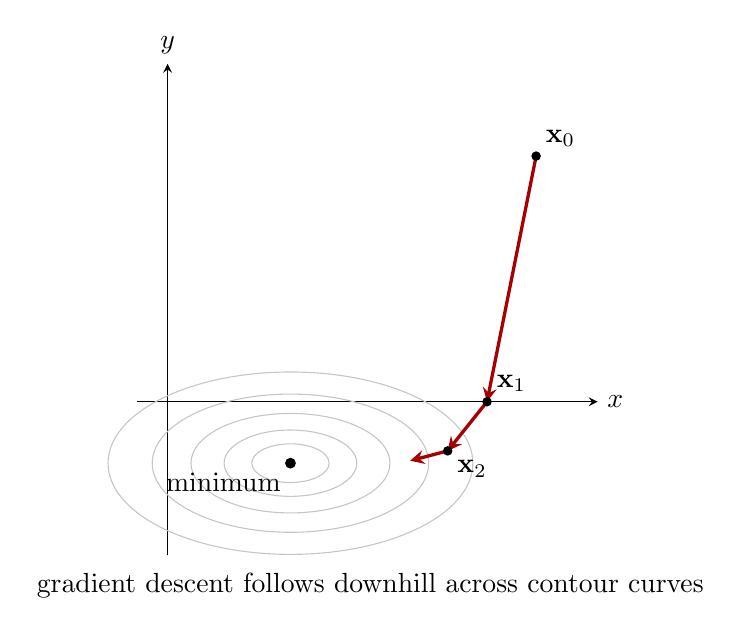
\begin{tikzpicture}[scale=0.78, >=stealth]
    \draw[->] (-0.5,0) -- (7,0) node[right] {\(x\)};
    \draw[->] (0,-2.5) -- (0,5.5) node[above] {\(y\)};

    \foreach \r in {0.7,1.2,1.8,2.5,3.3} {
        \draw[gray!45] (2,-1) ellipse ({0.9*\r} and {0.45*\r});
    }

    \coordinate (A) at (6,4);
    \coordinate (B) at (5.2,0);
    \coordinate (C) at (4.56,-0.8);
    \coordinate (D) at (3.95,-0.96);
    \coordinate (M) at (2,-1);

    \draw[->, very thick, red!65!black] (A) -- (B);
    \draw[->, very thick, red!65!black] (B) -- (C);
    \draw[->, very thick, red!65!black] (C) -- (D);

    \fill (A) circle (2.2pt) node[above right] {\(\mathbf x_0\)};
    \fill (B) circle (2.2pt) node[above right] {\(\mathbf x_1\)};
    \fill (C) circle (2.2pt) node[below right] {\(\mathbf x_2\)};
    \fill (M) circle (2.5pt) node[below left] {minimum};

    \node at (3.3,-3.0) {gradient descent follows downhill across contour curves};
\end{tikzpicture}
\caption{Gradient descent takes repeated steps in the negative-gradient direction.}
\end{figure}

\subsubsection*{Why step size matters}

Even in one variable, the step size can break the method.

Let
\[
    f(x)=x^2.
\]
Then
\[
    f'(x)=2x.
\]
Gradient descent gives
\[
    x_{n+1}=x_n-\alpha(2x_n)=(1-2\alpha)x_n.
\]
If
\[
    0<\alpha<1,
\]
then
\[
    |1-2\alpha|<1
\]
as long as \(\alpha\ne1\), and the iterates move toward \(0\).

If
\[
    \alpha=1,
\]
then
\[
    x_{n+1}=-x_n.
\]
The sequence bounces back and forth forever.

If
\[
    \alpha>1,
\]
then
\[
    |1-2\alpha|>1,
\]
and the iterates grow in size.  The method runs away from the minimum.

The direction was right, but the step was too large.

\subsubsection*{Your task}

Choose one function from Group A and one from Group B.

\subsubsection*{Group A: friendly quadratic bowls}

\[
\begin{array}{c}
f_1(x,y)=\frac12(x-2)^2+2(y+1)^2,\\[2mm]
f_2(x,y)=x^2+xy+y^2-4x-2y,\\[1mm]
f_3(x,y)=3(x+1)^2+(y-2)^2.
\end{array}
\]

\subsubsection*{Group B: functions with warnings}

\[
\begin{array}{c}
g_1(x,y)=x^2-y^2,\\[1mm]
g_2(x,y)=x^4+y^4-4xy,\\[1mm]
g_3(x,y)=\sin x+\cos y.
\end{array}
\]

For each function:

\begin{enumerate}
\item Compute the gradient.

\item Choose a starting point.

\item Choose a step size \(\alpha\).

\item Compute at least five gradient descent steps by hand, spreadsheet, calculator, or
code.

\item Plot the contour map and draw the step path.

\item Record the function values
\[
    f(\mathbf x_0),\ f(\mathbf x_1),\ f(\mathbf x_2),\ldots
\]
or
\[
    g(\mathbf x_0),\ g(\mathbf x_1),\ g(\mathbf x_2),\ldots
\]

\item Try a smaller step size and a larger step size.  Compare what happens.
\end{enumerate}

\subsubsection*{Questions to answer}

\begin{enumerate}
\item Did the function value decrease at every step?

\item Did the points appear to approach a minimum?

\item Did a large step size cause bouncing or divergence?

\item What happened for a saddle-shaped function such as
\[
    g_1(x,y)=x^2-y^2?
\]

\item How does the Hessian help explain the behavior near a critical point?
\end{enumerate}

\subsubsection*{What to hand in}

Your report should include:

\begin{enumerate}
\item the two functions you chose,

\item the gradients,

\item the starting points and step sizes,

\item a table of iterates,

\item a table of function values,

\item contour plots with the descent path drawn,

\item a paragraph explaining what worked and what failed.
\end{enumerate}

Gradient descent is simple enough to write in one line, but it is not magic.  It listens
only to local slope.  If the landscape has a saddle, a flat valley, many wells, or a step
size that is too large, the path can surprise us.

Optimization chooses best points.  Integration asks a different kind of question: not
where a quantity is largest or smallest, but how much of it is spread across a region.
The next group of projects returns to the adding machines of Chapters
\ref{ch:10}--\ref{ch:12}: double integrals, triple integrals, and change of variables.
% =====================================================================
%  Chapter 20: Capstone Projects and Extended Explorations
%  Sections 20.3 and 20.4
% =====================================================================

\section{Integration projects}
\label{sec:20.3}

Optimization chose best points.  Integration asks a different question:

\[
    \text{How much is spread over the whole region?}
\]

That region may be a plate, a room, a pond, a solid object, or a distorted image.  The
same idea keeps returning.  Cut the region into small pieces.  Estimate the contribution
from each piece.  Add.

\[
    \text{small contribution}
    =
    \text{value on the piece}\times \text{size of the piece}.
\]

These projects turn that sentence into measurements.

\subsection{Project 1: estimate mass from measured density data}

A formula is not always available.  Sometimes the density is known only from
measurements.

A lab technician may test a metal plate at several points.  A geologist may sample soil
density at grid locations.  A medical scan may give density values one voxel at a time.
The integral is still the right idea, but the integral has to be estimated from data.

\subsubsection*{A seed example: a nonuniform plate}

A thin rectangular plate occupies

\[
    0\le x\le6,
    \qquad
    0\le y\le4,
\]
where \(x\) and \(y\) are measured in centimeters.

The plate is divided into \(3\) columns and \(2\) rows.  Each small rectangle has width
\(2\) and height \(2\), so

\[
    \Delta A=4\text{ cm}^2.
\]

The density, measured in grams per square centimeter, is sampled at the center of each
small rectangle:

\[
\begin{array}{c|ccc}
 & x=1 & x=3 & x=5 \\ \hline
y=3 & 2.4 & 2.8 & 3.1\\
y=1 & 2.0 & 2.3 & 2.6
\end{array}
\]

The mass is

\[
    M=\iint_R \rho(x,y)\,dA.
\]

Using the midpoint rule, we estimate

\[
\begin{aligned}
M
&\approx
\sum \rho(x_i^*,y_j^*)\,\Delta A\\
&=
4(2.0+2.3+2.6+2.4+2.8+3.1)\\
&=
4(15.2)\\
&=
60.8.
\end{aligned}
\]

So the estimated mass is

\[
\boxed{
    M\approx 60.8\text{ g}.
}
\]

The area of the plate is

\[
    6\cdot4=24\text{ cm}^2.
\]
So the estimated average density is

\[
\boxed{
    \overline{\rho}
    =
    \frac{M}{\operatorname{Area}(R)}
    \approx
    \frac{60.8}{24}
    \approx
    2.53\text{ g/cm}^2.
}
\]

\begin{figure}[h]
\centering
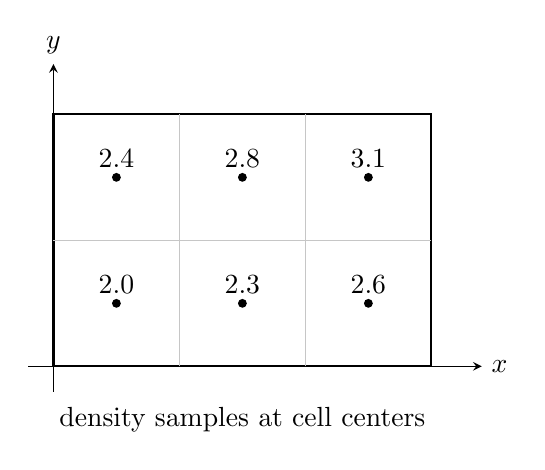
\begin{tikzpicture}[scale=0.8, >=stealth]
    \draw[->] (-0.4,0) -- (6.8,0) node[right] {\(x\)};
    \draw[->] (0,-0.4) -- (0,4.8) node[above] {\(y\)};

    \draw[thick] (0,0) rectangle (6,4);
    \draw[gray!45] (2,0) -- (2,4);
    \draw[gray!45] (4,0) -- (4,4);
    \draw[gray!45] (0,2) -- (6,2);

    \foreach \x/\y/\d in {
        1/1/2.0,
        3/1/2.3,
        5/1/2.6,
        1/3/2.4,
        3/3/2.8,
        5/3/3.1
    } {
        \fill (\x,\y) circle (2pt);
        \node[above] at (\x,\y) {\(\d\)};
    }

    \node at (3,-0.85) {density samples at cell centers};
\end{tikzpicture}
\caption{Measured density data can be turned into a mass estimate by a Riemann sum.}
\end{figure}

\subsubsection*{Your task}

Choose one of the following.

\subsubsection*{Option A. Plate from tabulated data}

Use the density table from the seed example, or create your own \(4\times4\) or
\(5\times5\) grid of density values.  Estimate the mass of the plate.

\subsubsection*{Option B. Temperature or pollution on a map}

Use a rectangular map region.  Let the data values represent temperature, pollution
concentration, or rainfall.  Estimate the total amount and the average value over the
region.

\subsubsection*{Option C. Three-dimensional density data}

A box is divided into small rectangular boxes.  At the center of each box, a density
value is measured.  Estimate

\[
    M=\iiint_E \rho(x,y,z)\,dV.
\]

For a simple version, use a \(2\times2\times2\) grid.

\subsubsection*{Required steps}

\begin{enumerate}
\item Draw the region and the sampling grid.

\item State the units of the density.

\item State the area or volume of each small piece:
\[
    \Delta A
    \qquad\text{or}\qquad
    \Delta V.
\]

\item Write the Riemann sum:
\[
    \sum \rho(x_i^*,y_i^*)\,\Delta A
\]
or
\[
    \sum \rho(x_i^*,y_i^*,z_i^*)\,\Delta V.
\]

\item Estimate the total mass or total amount.

\item Estimate the average density:
\[
    \overline{\rho}
    =
    \frac{\text{total amount}}{\text{area or volume}}.
\]

\item Discuss whether the estimate should improve with a finer grid.
\end{enumerate}

\subsubsection*{Questions to answer}

\begin{enumerate}
\item Which parts of the region have the largest density?

\item Does the data suggest a smooth density field or a sharp jump?

\item If one measurement were wrong, which one would most affect the estimate?

\item What changes if the data are sampled at corners instead of centers?

\item How would your estimate change if the grid cells had unequal sizes?
\end{enumerate}

\subsubsection*{What to hand in}

Your report should include:

\begin{enumerate}
\item the data table,

\item a grid drawing,

\item the Riemann sum,

\item the estimated total amount,

\item the estimated average value,

\item one paragraph explaining the main source of error.
\end{enumerate}

The main point is that an integral can survive without a formula.  A formula is one way
to know a field.  Measurements are another.

\subsection{Project 2: moments of inertia of real objects}

Mass tells how much material an object has.  Moment of inertia tells how that mass is
spread around an axis.

A heavy object is harder to spin if more of its mass is far from the axis.  That is why a
figure skater spins faster when pulling in her arms.  The mass has not changed, but the
mass has moved closer to the rotation axis.

The integral measures this spreading.

\[
\boxed{
    I=\int (\text{distance to axis})^2\,dm.
}
\]

For a thin plate with density \(\delta(x,y)\), this becomes

\[
\boxed{
    I=\iint_R (\text{distance to axis})^2\,\delta(x,y)\,dA.
}
\]

\subsubsection*{A seed example: a rectangular tray}

A rectangular tray is \(4\) meters long and \(2\) meters wide.  Put its center at the
origin, so the tray occupies

\[
    -2\le x\le2,
    \qquad
    -1\le y\le1.
\]

Suppose the tray has constant areal density

\[
    \delta=0.5\text{ kg/m}^2.
\]

Find the moment of inertia about the vertical axis through its center.

The distance from the point \((x,y)\) to the vertical axis is

\[
    r=\sqrt{x^2+y^2}.
\]
So

\[
    r^2=x^2+y^2.
\]

Thus

\[
\begin{aligned}
I_z
&=
\iint_R (x^2+y^2)\delta\,dA\\
&=
0.5\int_{-2}^{2}\int_{-1}^{1}(x^2+y^2)\,dy\,dx.
\end{aligned}
\]

Separate the integral:

\[
\begin{aligned}
I_z
&=
0.5\left(
\int_{-2}^{2}\int_{-1}^{1}x^2\,dy\,dx
+
\int_{-2}^{2}\int_{-1}^{1}y^2\,dy\,dx
\right)\\
&=
0.5\left(
\int_{-2}^{2}2x^2\,dx
+
\int_{-2}^{2}\frac{2}{3}\,dx
\right)\\
&=
0.5\left(
2\cdot\frac{16}{3}
+
\frac{2}{3}\cdot4
\right)\\
&=
0.5\left(
\frac{32}{3}+\frac{8}{3}
\right)\\
&=
\frac{20}{3}.
\end{aligned}
\]

So

\[
\boxed{
    I_z=\frac{20}{3}\text{ kg}\cdot\text{m}^2.
}
\]

The tray's mass is

\[
    M=0.5(4)(2)=4\text{ kg}.
\]

The radius of gyration is the distance \(R_g\) that would give the same moment of
inertia if all the mass were concentrated on a circle:

\[
    I_z=MR_g^2.
\]
Thus

\[
    R_g=\sqrt{\frac{I_z}{M}}
    =
    \sqrt{\frac{20/3}{4}}
    =
    \sqrt{\frac53}.
\]

This number is not the physical radius of the tray.  It is a weighted average distance
from the axis.

\begin{figure}[h]
\centering
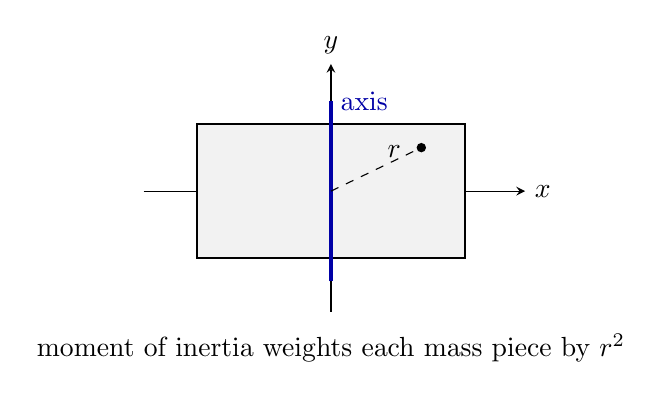
\begin{tikzpicture}[scale=0.85, >=stealth]
    \draw[->] (-2.8,0) -- (2.9,0) node[right] {\(x\)};
    \draw[->] (0,-1.8) -- (0,1.9) node[above] {\(y\)};

    \draw[fill=gray!10, thick] (-2,-1) rectangle (2,1);

    \draw[very thick, blue!65!black] (0,-1.35) -- (0,1.35);
    \node[blue!65!black, right] at (0,1.35) {axis};

    \fill (1.35,0.65) circle (2pt);
    \draw[dashed] (0,0) -- (1.35,0.65);
    \node[above right] at (0.7,0.35) {\(r\)};

    \node at (0,-2.35) {moment of inertia weights each mass piece by \(r^2\)};
\end{tikzpicture}
\caption{Mass farther from the axis contributes more to moment of inertia.}
\end{figure}

\subsubsection*{Your task}

Choose one object or model.

\subsubsection*{Option A. Uniform rectangular plate}

Compute the moment of inertia of a rectangular plate about one of its symmetry axes
and about the axis perpendicular to the plate through its center.

\subsubsection*{Option B. Disk or annulus}

Use polar coordinates to compute the moment of inertia of a uniform disk or annulus
about its central axis.

\subsubsection*{Option C. Triangular lamina}

Choose a triangular region in the plane.  Compute its mass and moment of inertia using
double integrals.

\subsubsection*{Option D. Measured object}

Approximate a real flat object by dividing it into small pieces.  Estimate each piece's
mass and distance from the chosen axis.  Use the discrete approximation

\[
    I\approx \sum r_i^2\,\Delta m_i.
\]

\subsubsection*{Option E. Solid object}

Compute or estimate the moment of inertia of a solid cylinder, rectangular box, or ball
using a triple integral.

\subsubsection*{Required steps}

\begin{enumerate}
\item Draw the object and the rotation axis.

\item State whether the density is constant or variable.

\item Write the distance squared to the axis.

\item Set up the integral:
\[
    I=\iint_R r^2\delta\,dA
\]
or
\[
    I=\iiint_E r^2\rho\,dV.
\]

\item Choose coordinates that make the integral simpler.

\item Compute the mass.

\item Compute the moment of inertia.

\item Interpret the answer physically.
\end{enumerate}

\subsubsection*{Questions to answer}

\begin{enumerate}
\item Which parts of the object contribute most to \(I\)?

\item What happens if the same mass is moved farther from the axis?

\item Does symmetry simplify the integral?

\item Can you verify your answer using the perpendicular-axis theorem or the
parallel-axis theorem, where appropriate?

\item How would the answer change if the density were larger near the edge?
\end{enumerate}

\subsubsection*{What to hand in}

Your report should include:

\begin{enumerate}
\item a labeled diagram,

\item the density model,

\item the chosen axis,

\item the moment-of-inertia integral,

\item the calculation,

\item the final value with units,

\item a physical explanation of why the answer is reasonable.
\end{enumerate}

Moment of inertia is an integral with a memory of distance.  A mass piece does not
only count by how much mass it has.  It counts by where it sits.

\subsection{Project 3: change of variables in image warping}

A change of variables is a controlled distortion.

In Chapter \ref{ch:12}, a coordinate map sent tiny squares in one coordinate plane to
tiny parallelograms in another.  The determinant measured how the area changed.  The
same idea appears in image warping.  A square image may be stretched, sheared,
wrapped, or bent.  If we want to compute area, brightness, or ink after the warp, the
Jacobian must be included.

\subsubsection*{A seed example: a square stretched into a trapezoid}

Start with the unit square

\[
    0\le u\le1,
    \qquad
    0\le v\le1.
\]

Define a map

\[
    T(u,v)=(x,y)=\bigl(u,\,(1+u)v\bigr).
\]

When \(u=0\), the vertical height is \(1\).  When \(u=1\), the vertical height is \(2\).
So the square is warped into a trapezoid.

The tangent vectors are

\[
    T_u=(1,v),
    \qquad
    T_v=(0,1+u).
\]

The Jacobian determinant is

\[
\begin{aligned}
J(u,v)
&=
\det
\begin{pmatrix}
x_u & x_v\\
y_u & y_v
\end{pmatrix}       \\
&=
\det
\begin{pmatrix}
1&0\\
v&1+u
\end{pmatrix}\\
&=
1+u.
\end{aligned}
\]

So a tiny square of area \(du\,dv\) becomes a tiny region of area approximately

\[
    (1+u)\,du\,dv.
\]

The area of the warped image is

\[
\begin{aligned}
\operatorname{Area}
&=
\int_0^1\int_0^1 (1+u)\,dv\,du\\
&=
\int_0^1(1+u)\,du\\
&=
\frac32.
\end{aligned}
\]

That matches the ordinary trapezoid formula:

\[
    \frac12(1+2)(1)=\frac32.
\]

Now suppose the brightness of the warped image is

\[
    B(x,y)=x+y.
\]
Then the total brightness is

\[
    \iint_{\text{warped image}} B(x,y)\,dA.
\]

Using the change of variables,

\[
\begin{aligned}
\iint_{\text{warped image}} B\,dA
&=
\int_0^1\int_0^1
B(T(u,v))\,|J(u,v)|\,dv\,du\\
&=
\int_0^1\int_0^1
\bigl(u+(1+u)v\bigr)(1+u)\,dv\,du.
\end{aligned}
\]

Compute the inner integral:

\[
\begin{aligned}
\int_0^1
\bigl(u+(1+u)v\bigr)(1+u)\,dv
&=
u(1+u)+\frac12(1+u)^2.
\end{aligned}
\]

Then

\[
\begin{aligned}
\int_0^1
\left[
u(1+u)+\frac12(1+u)^2
\right]du
&=
\int_0^1
\left(
\frac12+2u+\frac32u^2
\right)du\\
&=
\frac12+1+\frac12\\
&=
2.
\end{aligned}
\]

So

\[
\boxed{
    \iint_{\text{warped image}}(x+y)\,dA=2.
}
\]

\begin{figure}[h]
\centering
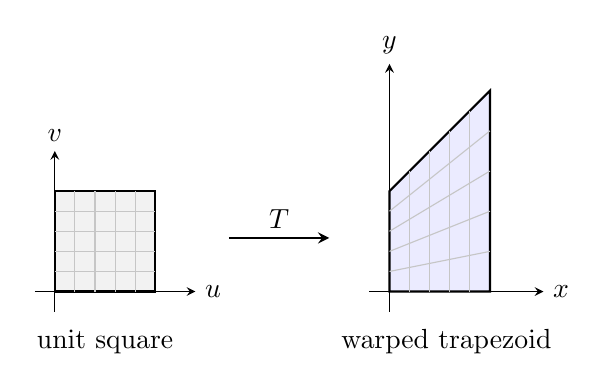
\begin{tikzpicture}[scale=0.85, >=stealth]
    \begin{scope}
        \draw[->] (-0.3,0) -- (2.1,0) node[right] {\(u\)};
        \draw[->] (0,-0.3) -- (0,2.1) node[above] {\(v\)};

        \draw[fill=gray!10, thick] (0,0) rectangle (1.5,1.5);

        \foreach \x in {0.3,0.6,0.9,1.2} {
            \draw[gray!45] (\x,0) -- (\x,1.5);
        }
        \foreach \y in {0.3,0.6,0.9,1.2} {
            \draw[gray!45] (0,\y) -- (1.5,\y);
        }

        \node at (0.75,-0.75) {unit square};
    \end{scope}

    \draw[->, thick] (2.6,0.8) -- (4.1,0.8);
    \node[above] at (3.35,0.8) {\(T\)};

    \begin{scope}[shift={(5.0,0)}]
        \draw[->] (-0.3,0) -- (2.3,0) node[right] {\(x\)};
        \draw[->] (0,-0.3) -- (0,3.4) node[above] {\(y\)};

        \draw[fill=blue!8, thick] (0,0) -- (1.5,0) -- (1.5,3.0) -- (0,1.5) -- cycle;

        \foreach \u in {0.3,0.6,0.9,1.2} {
            \draw[gray!45] (\u,0) -- (\u,{1.5*(1+\u/1.5)});
        }

        \foreach \v in {0.3,0.6,0.9,1.2} {
            \draw[gray!45] (0,\v) -- (1.5,{2*\v});
        }

        \node at (0.85,-0.75) {warped trapezoid};
    \end{scope}
\end{tikzpicture}
\caption{A coordinate warp changes the area of small grid cells.  The Jacobian records
the local area scale.}
\end{figure}

\subsubsection*{Your task}

Choose one map \(T\) from the list or create your own.

\[
\begin{array}{c|c}
\text{Name} & T(u,v)=(x,y) \\ \hline
\text{shear} & (u+av,\ v)\\[1mm]
\text{stretch} & (au,\ bv)\\[1mm]
\text{trapezoid warp} & (u,\ (1+u)v)\\[1mm]
\text{fold warning} & (u^2,\ v)\\[1mm]
\text{polar annulus} & ((1+r)\cos\theta,\ (1+r)\sin\theta)
\end{array}
\]

For the polar annulus, use

\[
    0\le r\le1,
    \qquad
    0\le\theta\le2\pi.
\]

\subsubsection*{Required steps}

\begin{enumerate}
\item Draw the parameter region.

\item Draw or plot the warped image.

\item Compute the tangent vectors:
\[
    T_u,\qquad T_v.
\]

\item Compute the Jacobian determinant:
\[
    J=\det
    \begin{pmatrix}
    x_u & x_v\\
    y_u & y_v
    \end{pmatrix}.
\]

\item Decide whether the map preserves orientation, reverses orientation, or changes
sign somewhere.

\item Compute the area of the image:
\[
    \iint_D |J|\,du\,dv.
\]

\item Choose a simple brightness function \(B(x,y)\), such as
\[
    B(x,y)=1,\qquad B(x,y)=x,\qquad B(x,y)=x+y,
\]
and compute
\[
    \iint_{\text{image}}B(x,y)\,dA
\]
using the pullback:
\[
    \iint_D B(T(u,v))\,|J(u,v)|\,du\,dv.
\]
\end{enumerate}

\subsubsection*{Questions to answer}

\begin{enumerate}
\item Where does the map stretch area the most?

\item Where does it shrink area?

\item Does the map ever collapse a two-dimensional region into a curve?

\item Does the sign of \(J\) matter for ordinary area?

\item Where would the sign of \(J\) matter for an oriented integral such as
\[
    \iint f\,dx\wedge dy?
\]
\end{enumerate}

\subsubsection*{What to hand in}

Your report should include:

\begin{enumerate}
\item the coordinate map,

\item a picture of the parameter grid and the warped grid,

\item the Jacobian calculation,

\item the area calculation,

\item one pulled-back integral,

\item a paragraph explaining what the Jacobian means geometrically.
\end{enumerate}

A warped image is a friendly place to see the change-of-variables formula.  The picture
changes shape, but the integral stays honest because the Jacobian keeps track of the
stretching.

\subsection{Project 4: Monte Carlo integration in two and three dimensions}

Some regions are too irregular for clean limits.  Some functions are known only through
simulation.  Some dimensions are too high for ordinary grid methods to be practical.

Monte Carlo integration uses random samples instead of a regular grid.

The idea is simple: average many random values, then multiply by the size of the
sampling box.

\subsubsection*{A seed example: estimating water volume in a circular pond}

A shallow circular pond has radius \(2\).  Its depth is modeled by

\[
    d(x,y)=5-x^2-y^2
\]
inside the disk

\[
    D=\{(x,y):x^2+y^2\le4\}.
\]

The volume of water is

\[
    V=\iint_D (5-x^2-y^2)\,dA.
\]

We could use polar coordinates:

\[
\begin{aligned}
V
&=
\int_0^{2\pi}\int_0^2(5-r^2)r\,dr\,d\theta\\
&=
2\pi
\left[
\frac52r^2-\frac14r^4
\right]_0^2\\
&=
2\pi(10-4)\\
&=
12\pi.
\end{aligned}
\]

So the exact volume is approximately

\[
    37.70.
\]

Now estimate the same integral by Monte Carlo sampling.  Put the pond inside the square

\[
    B=[-2,2]\times[-2,2].
\]
The square has area \(16\).

Define

\[
    g(x,y)=
    \begin{cases}
    5-x^2-y^2, & x^2+y^2\le4,\\
    0, & x^2+y^2>4.
    \end{cases}
\]

Then

\[
    \iint_D(5-x^2-y^2)\,dA
    =
    \iint_B g(x,y)\,dA.
\]

Suppose five random points in \(B\) give the following values:

\[
\begin{array}{c|c|c}
(x,y) & x^2+y^2 & g(x,y) \\ \hline
(0.4,-1.1) & 1.37 & 3.63\\
(-1.8,0.6) & 3.60 & 1.40\\
(1.7,1.5) & 5.14 & 0\\
(-0.2,0.3) & 0.13 & 4.87\\
(1.1,-0.7) & 1.70 & 3.30
\end{array}
\]

The sample average is

\[
    \frac{3.63+1.40+0+4.87+3.30}{5}=2.64.
\]

So the Monte Carlo estimate is

\[
\boxed{
    V\approx 16(2.64)=42.24.
}
\]

That is rough, because \(N=5\) is tiny.  With hundreds or thousands of samples, the
estimate should settle closer to \(12\pi\).

\subsubsection*{The general Monte Carlo formula}

Let \(E\) be a region inside a box \(B\).  Define

\[
    g(\mathbf x)=
    \begin{cases}
    f(\mathbf x), & \mathbf x\in E,\\
    0, & \mathbf x\notin E.
    \end{cases}
\]

If

\[
    \mathbf X_1,\mathbf X_2,\ldots,\mathbf X_N
\]
are random points chosen uniformly in \(B\), then

\[
\boxed{
    \int_E f
    \approx
    \operatorname{size}(B)\,
    \frac{1}{N}
    \sum_{i=1}^{N} g(\mathbf X_i).
}
\]

Here \(\operatorname{size}(B)\) means area in two dimensions and volume in three
dimensions.

\subsubsection*{Your task}

Choose one integral.

\subsubsection*{Option A. Area of an irregular region}

Estimate the area of a region \(E\) by taking

\[
    f=1.
\]

\subsubsection*{Option B. Volume under a surface}

Estimate

\[
    \iint_E f(x,y)\,dA
\]
for a region \(E\) inside a rectangle.

\subsubsection*{Option C. Mass inside a solid}

Estimate

\[
    \iiint_E \rho(x,y,z)\,dV
\]
for a solid \(E\) inside a box.

\subsubsection*{Option D. Compare Monte Carlo with an exact answer}

Choose an integral that can also be computed exactly, such as a disk, ball, cylinder, or
box.  Compare the Monte Carlo estimate with the exact value.

\subsubsection*{Required steps}

\begin{enumerate}
\item State the region \(E\).

\item Choose a sampling box \(B\).

\item Define the function \(g\) on the whole box.

\item Generate random sample points.

\item Compute the estimate for several values of \(N\), such as
\[
    N=100,\quad 500,\quad 1000,\quad 5000.
\]

\item Plot or tabulate the estimates as \(N\) grows.

\item Compare with an exact or high-resolution numerical answer, if available.
\end{enumerate}

\subsubsection*{Questions to answer}

\begin{enumerate}
\item Does the estimate appear to converge?

\item How much does the answer change when you run the experiment again?

\item What happens if the sampling box is much larger than the region \(E\)?

\item Why are points outside \(E\) assigned value \(0\)?

\item What advantage does random sampling have in three dimensions?
\end{enumerate}

\subsubsection*{What to hand in}

Your report should include:

\begin{enumerate}
\item the integral being estimated,

\item the sampling box,

\item the Monte Carlo formula used,

\item a table of estimates for increasing \(N\),

\item a plot of the estimates, if possible,

\item a comparison with an exact or more accurate value,

\item a paragraph about reliability and error.
\end{enumerate}

The integration projects mostly add scalar quantities: density, brightness, mass,
volume, and moment.  Vector calculus adds direction.  A force pushes along a path.  A
fluid crosses a surface.  A boundary can reveal an area, and a flux balance can reveal a
source.  The next projects return to the book's boundary theme.

\section{Vector calculus projects}
\label{sec:20.4}

The previous projects added quantities over regions.  Vector calculus asks what happens
along boundaries and through surfaces.  Work follows curves.  Flux crosses surfaces.
Green's theorem, Stokes' theorem, and the divergence theorem say that boundary
measurements can reveal interior information.

The projects below are meant to make that principle measurable.

\subsection{Project 1: work around closed curves}

A closed curve returns to where it started.  A conservative field does no net work
around such a curve.  A rotating field may do positive or negative work, depending on
the direction of travel.

The line integral detects the difference.

\subsubsection*{A seed example: a field that measures area}

Let

\[
    \mathbf F(x,y)=\left(-\frac y2,\frac x2\right),
\]
and let

\[
    \omega=-\frac y2\,dx+\frac x2\,dy
\]
be its work \(1\)-form.

Walk counterclockwise around the rectangle

\[
    R=[0,4]\times[0,3].
\]

We compute the work around the four sides.

\subsubsection*{Bottom side}

Here \(y=0\) and \(dy=0\).  So

\[
    \omega=0.
\]
The bottom contributes \(0\).

\subsubsection*{Right side}

Here \(x=4\), \(dx=0\), and \(y\) goes from \(0\) to \(3\).  Thus

\[
\begin{aligned}
\int_{\text{right}}\omega
&=
\int_0^3 \frac{4}{2}\,dy\\
&=
6.
\end{aligned}
\]

\subsubsection*{Top side}

Here \(y=3\), \(dy=0\), and \(x\) goes from \(4\) back to \(0\).  Thus

\[
\begin{aligned}
\int_{\text{top}}\omega
&=
\int_4^0 -\frac32\,dx\\
&=
6.
\end{aligned}
\]

\subsubsection*{Left side}

Here \(x=0\), \(dx=0\), and \(y\) goes downward.  Thus

\[
    \omega=0.
\]
The left side contributes \(0\).

So

\[
\boxed{
    \oint_{\partial R}\omega=12.
}
\]

The rectangle has area

\[
    4\cdot3=12.
\]

This is not a coincidence.  Compute the exterior derivative:

\[
\begin{aligned}
d\omega
&=
d\left(-\frac y2\,dx+\frac x2\,dy\right)\\
&=
\left(\frac{\partial}{\partial x}\frac x2
-
\frac{\partial}{\partial y}\left(-\frac y2\right)
\right)dx\wedge dy\\
&=
\left(\frac12+\frac12\right)dx\wedge dy\\
&=
dx\wedge dy.
\end{aligned}
\]

Green's theorem gives

\[
\boxed{
    \oint_{\partial R}\omega
    =
    \iint_R d\omega
    =
    \iint_R dx\wedge dy
    =
    \operatorname{Area}(R).
}
\]

The work form is secretly an area-measuring instrument.

\begin{figure}[h]
\centering
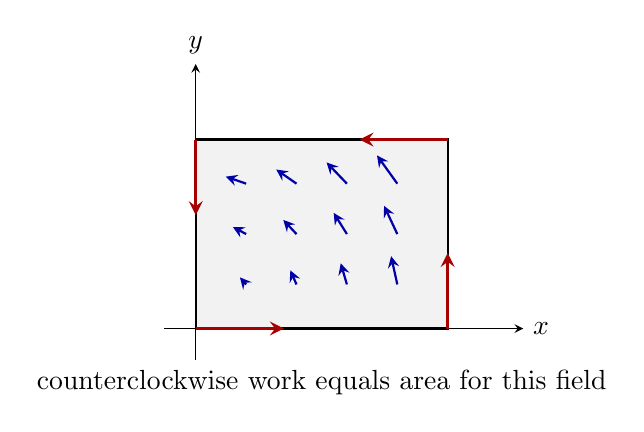
\begin{tikzpicture}[scale=0.8, >=stealth]
    \draw[->] (-0.5,0) -- (5.2,0) node[right] {\(x\)};
    \draw[->] (0,-0.5) -- (0,4.2) node[above] {\(y\)};

    \draw[fill=gray!10, thick] (0,0) rectangle (4,3);

    \draw[->, very thick, red!65!black] (0,0) -- (1.4,0);
    \draw[->, very thick, red!65!black] (4,0) -- (4,1.2);
    \draw[->, very thick, red!65!black] (4,3) -- (2.6,3);
    \draw[->, very thick, red!65!black] (0,3) -- (0,1.8);

    \foreach \x in {0.8,1.6,2.4,3.2} {
        \foreach \y in {0.7,1.5,2.3} {
            \draw[->, blue!65!black, thick]
                (\x,\y) -- ++({-0.14*\y},{0.14*\x});
        }
    }

    \node at (2,-0.85) {counterclockwise work equals area for this field};
\end{tikzpicture}
\caption{A rotational field can do positive work around a closed curve.}
\end{figure}

\subsubsection*{Your task}

Choose one field and one closed curve.

\[
\begin{array}{c|c}
\text{Field} & \text{Feature} \\ \hline
\mathbf F=(-y,x) & \text{constant positive scalar curl }2\\[1mm]
\mathbf F=\left(-\dfrac y2,\dfrac x2\right) & \text{work equals area}\\[4mm]
\mathbf F=(2x,2y) & \text{gradient field}\\[1mm]
\mathbf F=(y^2,x) & \text{nonconstant scalar curl}\\[1mm]
\mathbf F=\left(\dfrac{-y}{x^2+y^2},\dfrac{x}{x^2+y^2}\right)
& \text{punctured-plane warning}
\end{array}
\]

For curves, use a circle, ellipse, rectangle, triangle, or a piecewise smooth curve of
your own.

\subsubsection*{Required steps}

\begin{enumerate}
\item Draw the vector field and the closed curve.

\item Choose an orientation for the curve.

\item Write the work form
\[
    \omega=P\,dx+Q\,dy.
\]

\item Compute the line integral directly, if possible.

\item Compute
\[
    d\omega=(Q_x-P_y)\,dx\wedge dy.
\]

\item Use Green's theorem if the field is defined on the region enclosed by the curve.

\item Compare the direct calculation with the theorem calculation.

\item Reverse the curve orientation and state what changes.
\end{enumerate}

\subsubsection*{Questions to answer}

\begin{enumerate}
\item Is the work positive, negative, or zero?

\item Does the field help the chosen direction of travel?

\item Is the field a gradient field?

\item If the field has zero curl away from a missing point, can the closed integral still
be nonzero?

\item What does the answer say about the domain?
\end{enumerate}

\subsubsection*{What to hand in}

Your report should include:

\begin{enumerate}
\item the chosen field and curve,

\item the parametrization of the curve,

\item the line integral,

\item the exterior derivative \(d\omega\),

\item the Green's theorem calculation, when allowed,

\item a paragraph explaining the role of orientation and domain holes.
\end{enumerate}

A closed curve can hide a surprise.  Even if every local test looks harmless, a missing
point inside the loop can change the answer.

\subsection{Project 2: flux through complicated surfaces}

Flux measures how much a vector field crosses a surface.  A flat disk is friendly.  A
curved dome is less friendly.  A surface made of several pieces can look intimidating.

The divergence theorem offers a shortcut, but only after the surface is closed.

\subsubsection*{A seed example: flux through a paraboloid dome}

Let \(S\) be the dome

\[
    z=4-x^2-y^2,
    \qquad
    x^2+y^2\le4,
\]
oriented upward.  Together with the disk

\[
    D:\quad z=0,\qquad x^2+y^2\le4,
\]
the dome bounds a solid \(E\).

Let

\[
    \mathbf F(x,y,z)=(x,y,z).
\]

We want the flux through the dome \(S\).

The closed surface is

\[
    \partial E=S\cup D,
\]
with outward orientation.  On the dome, outward means upward and outward.  On the
bottom disk, outward means downward.

The divergence is

\[
    \nabla\cdot\mathbf F
    =
    1+1+1
    =
    3.
\]

By the divergence theorem,

\[
    \iint_{\partial E}\mathbf F\cdot\widehat{\mathbf n}\,dS
    =
    \iiint_E 3\,dV
    =
    3\operatorname{Volume}(E).
\]

Find the volume of \(E\):

\[
\begin{aligned}
\operatorname{Volume}(E)
&=
\int_0^{2\pi}\int_0^2(4-r^2)r\,dr\,d\theta\\
&=
2\pi\left[
2r^2-\frac14r^4
\right]_0^2\\
&=
2\pi(8-4)\\
&=
8\pi.
\end{aligned}
\]

So the total outward flux through the closed surface is

\[
    3(8\pi)=24\pi.
\]

Now check the bottom disk.  On \(D\),

\[
    z=0,
    \qquad
    \widehat{\mathbf n}=(0,0,-1).
\]
Thus

\[
    \mathbf F\cdot\widehat{\mathbf n}
    =
    (x,y,0)\cdot(0,0,-1)
    =
    0.
\]

So the bottom disk contributes \(0\).  Therefore the flux through the dome is

\[
\boxed{
    \iint_S \mathbf F\cdot\widehat{\mathbf n}\,dS=24\pi.
}
\]

In forms language, the flux form is

\[
    \Phi_{\mathbf F}
    =
    x\,dy\wedge dz
    +
    y\,dz\wedge dx
    +
    z\,dx\wedge dy,
\]
and

\[
    d\Phi_{\mathbf F}
    =
    3\,dx\wedge dy\wedge dz.
\]

The same computation says

\[
    \int_{\partial E}\Phi_{\mathbf F}
    =
    \int_E d\Phi_{\mathbf F}.
\]

\subsubsection*{Your task}

Choose one surface.

\[
\begin{array}{c|c}
\text{Surface} & \text{Suggested field} \\ \hline
\text{paraboloid cap} & (x,y,z)\\[1mm]
\text{hemisphere with disk base} & (0,0,z)\\[1mm]
\text{cylinder side plus caps} & (x,y,1)\\[1mm]
\text{box with one face removed} & (x^2,y,z)\\[1mm]
\text{triangulated surface or mesh} & \text{constant or radial field}
\end{array}
\]

\subsubsection*{Required steps}

\begin{enumerate}
\item Draw the surface and state its orientation.

\item Decide whether the surface is closed.

\item If it is not closed, add simple pieces to close it.

\item Compute the flux through the closed surface using the divergence theorem, if
possible.

\item Compute or subtract the flux through the added pieces.

\item State the flux through the original surface.

\item Translate the flux integral into a \(2\)-form:
\[
    \Phi_{\mathbf F}
    =
    F_1\,dy\wedge dz
    +
    F_2\,dz\wedge dx
    +
    F_3\,dx\wedge dy.
\]
\end{enumerate}

\subsubsection*{Questions to answer}

\begin{enumerate}
\item Is the surface open or closed?

\item What does ``outward'' mean for each piece?

\item Which pieces contribute zero flux by symmetry or by the direction of the field?

\item Is the divergence theorem faster than a direct surface integral?

\item What would change if the orientation were reversed?
\end{enumerate}

\subsubsection*{What to hand in}

Your report should include:

\begin{enumerate}
\item a drawing of the surface,

\item the vector field,

\item the orientation,

\item the closed-surface construction,

\item the divergence calculation,

\item the flux through any added pieces,

\item the final flux through the requested surface.
\end{enumerate}

A surface integral can be hard because the surface is curved.  The divergence theorem
moves the difficulty into the solid it bounds.  Sometimes the inside is easier than the
skin.

\subsection{Project 3: Green's theorem and area from GPS boundary data}

A region's area can be found without filling the region with a grid.  It can be found by
walking around the boundary.

Green's theorem explains why.

Let

\[
    \eta=\frac12(x\,dy-y\,dx).
\]
Then

\[
\begin{aligned}
d\eta
&=
\frac12(dx\wedge dy-dy\wedge dx)\\
&=
dx\wedge dy.
\end{aligned}
\]

So, for a positively oriented boundary,

\[
\boxed{
    \operatorname{Area}(R)
    =
    \oint_{\partial R}\frac12(x\,dy-y\,dx).
}
\]

This formula is the continuous version of the shoelace formula for polygons.

\subsubsection*{A seed example: four boundary points}

Suppose a surveyor records four boundary points of a small field, measured in meters
from a local reference point:

\[
\begin{array}{c|cc}
\text{Point} & x & y \\ \hline
P_0 & 0 & 0\\
P_1 & 5 & 1\\
P_2 & 4 & 4\\
P_3 & 1 & 3
\end{array}
\]

Assume the points are listed counterclockwise and connected by straight segments.

On a line segment from

\[
    (x_i,y_i)
\]
to

\[
    (x_{i+1},y_{i+1}),
\]
the integral of \(\eta\) is

\[
\boxed{
    \frac12(x_i y_{i+1}-y_i x_{i+1}).
}
\]

Therefore

\[
\begin{aligned}
\operatorname{Area}
&=
\frac12\sum_{i=0}^{3}
(x_i y_{i+1}-y_i x_{i+1})\\
&=
\frac12\Bigl[
(0\cdot1-0\cdot5)
+
(5\cdot4-1\cdot4)\\
&\qquad
+
(4\cdot3-4\cdot1)
+
(1\cdot0-3\cdot0)
\Bigr]\\
&=
\frac12(0+16+8+0)\\
&=
12.
\end{aligned}
\]

So the field has area

\[
\boxed{
    12\text{ m}^2.
}
\]

If the points were listed clockwise, the same calculation would give

\[
    -12.
\]
The negative sign would not mean negative physical area.  It would mean the boundary
orientation was reversed.

\begin{figure}[h]
\centering
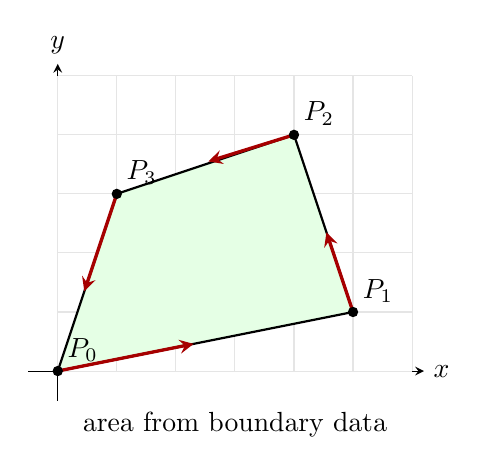
\begin{tikzpicture}[scale=0.75, >=stealth]
    \draw[->] (-0.5,0) -- (6.2,0) node[right] {\(x\)};
    \draw[->] (0,-0.5) -- (0,5.2) node[above] {\(y\)};

    \draw[gray!20, step=1] (0,0) grid (6,5);

    \draw[fill=green!10, thick] (0,0) -- (5,1) -- (4,4) -- (1,3) -- cycle;

    \draw[->, very thick, red!65!black] (0,0) -- (2.3,0.46);
    \draw[->, very thick, red!65!black] (5,1) -- (4.55,2.35);
    \draw[->, very thick, red!65!black] (4,4) -- (2.55,3.55);
    \draw[->, very thick, red!65!black] (1,3) -- (0.45,1.35);

    \foreach \p/\name in {(0,0)/P_0,(5,1)/P_1,(4,4)/P_2,(1,3)/P_3} {
        \fill \p circle (2.5pt);
        \node[above right] at \p {\(\name\)};
    }

    \node at (3,-0.9) {area from boundary data};
\end{tikzpicture}
\caption{Green's theorem turns a boundary walk into an area calculation.}
\end{figure}

\subsubsection*{Your task}

Choose one boundary data set.

\subsubsection*{Option A. Use provided data}

Use the four-point data from the seed example.  Then add more points to create a
six-point or eight-point polygon and compute its area.

\subsubsection*{Option B. Create a boundary}

Draw an irregular region on graph paper.  Record its boundary points in order.  Compute
the area using the shoelace formula.

\subsubsection*{Option C. Use local GPS-style data}

Record boundary points of a small region.  Convert the locations to local planar
coordinates measured in meters before using the formula.  Latitude and longitude
degrees are not distances.

\subsubsection*{Option D. Region with a hole}

Use an outer boundary and an inner boundary.  Orient the outer boundary
counterclockwise and the inner boundary clockwise.  Compute the area of the region
with the hole removed.

\subsubsection*{Required steps}

\begin{enumerate}
\item List the boundary points in order.

\item Plot the polygon.

\item Check the orientation.

\item Compute
\[
    \frac12\sum_i (x_i y_{i+1}-y_i x_{i+1}).
\]

\item Interpret the sign.

\item Compare with a rough grid-counting estimate.

\item Explain how this formula comes from Green's theorem:
\[
    \oint_{\partial R}\frac12(x\,dy-y\,dx)
    =
    \iint_R dx\wedge dy.
\]
\end{enumerate}

\subsubsection*{Questions to answer}

\begin{enumerate}
\item What happens if two boundary points are listed in the wrong order?

\item What happens if the boundary crosses itself?

\item How does the sign detect clockwise versus counterclockwise order?

\item Why must an inner boundary be oriented clockwise?

\item How accurate is the polygon area if the true boundary is curved?
\end{enumerate}

\subsubsection*{What to hand in}

Your report should include:

\begin{enumerate}
\item a table of boundary points,

\item a plot of the boundary,

\item the shoelace computation,

\item the area with units,

\item a Green's theorem explanation,

\item a short error discussion.
\end{enumerate}

This project is a good example of the book's main theme.  The area lies inside the
region, but the calculation only walks around the edge.

\subsection{Project 4: divergence theorem and numerical flux balance}

The divergence theorem says that outward flux through a closed surface equals total
divergence inside:

\[
\boxed{
    \iint_{\partial E}\mathbf J\cdot\widehat{\mathbf n}\,dS
    =
    \iiint_E \nabla\cdot\mathbf J\,dV.
}
\]

In Chapter \ref{ch:19}, this became a conservation law.  If \(\mathbf J\) is a flux
density, then outward flux is loss from the region unless sources replace it.

This project checks that balance numerically.

\subsubsection*{A seed example: flux through a unit cube}

Let

\[
    E=[0,1]\times[0,1]\times[0,1],
\]
and let

\[
    \mathbf J(x,y,z)=(x^2,y,z).
\]

First compute the divergence:

\[
    \nabla\cdot\mathbf J
    =
    2x+1+1
    =
    2x+2.
\]

The volume integral is

\[
\begin{aligned}
\iiint_E(2x+2)\,dV
&=
\int_0^1\int_0^1\int_0^1(2x+2)\,dz\,dy\,dx\\
&=
\int_0^1(2x+2)\,dx\\
&=
\left[x^2+2x\right]_0^1\\
&=
3.
\end{aligned}
\]

Now compute the outward flux through the six faces.

\[
\begin{array}{c|c|c|c}
\text{Face} & \widehat{\mathbf n} & \mathbf J\cdot\widehat{\mathbf n}
& \text{Flux} \\ \hline
x=1 & (1,0,0) & 1 & 1\\
x=0 & (-1,0,0) & 0 & 0\\
y=1 & (0,1,0) & 1 & 1\\
y=0 & (0,-1,0) & 0 & 0\\
z=1 & (0,0,1) & 1 & 1\\
z=0 & (0,0,-1) & 0 & 0
\end{array}
\]

So the total outward flux is

\[
    1+0+1+0+1+0=3.
\]

The two sides match:

\[
\boxed{
    \iint_{\partial E}\mathbf J\cdot\widehat{\mathbf n}\,dS
    =
    \iiint_E\nabla\cdot\mathbf J\,dV
    =
    3.
}
\]

\subsubsection*{Numerical flux balance}

In a numerical calculation, the two sides may not match exactly.  We can measure the
error by the residual

\[
\boxed{
    \mathcal R
    =
    \left(
    \text{estimated outward boundary flux}
    \right)
    -
    \left(
    \text{estimated interior divergence}
    \right).
}
\]

For an exact calculation,

\[
    \mathcal R=0.
\]
For a numerical calculation, a small residual means the discretization is respecting the
balance law well.  A large residual means that the grid, the data, or the orientation may
be wrong.



\subsubsection*{Your task}

Choose one version.

\subsubsection*{Option A. Exact cube check}

Use a rectangular box and a polynomial field.  Compute both sides exactly.

\subsubsection*{Option B. Numerical cube check}

Use midpoint or trapezoid sums on the six faces and inside the box.  Estimate both
sides and compute the residual.

\subsubsection*{Option C. Incompressible flow}

Choose a divergence-free field, such as

\[
    \mathbf J=(-y,x,0)
\]
or

\[
    \mathbf J=(yz,xz,xy)
\]
after checking its divergence.  Estimate the outward flux through a closed surface and
explain why it should be close to \(0\).

\subsubsection*{Option D. Flux balance with sources}

Use a source function \(s(x,y,z)\).  Compare the conservation law

\[
    \frac{d}{dt}\iiint_E\rho\,dV
    +
    \iint_{\partial E}\mathbf J\cdot\widehat{\mathbf n}\,dS
    =
    \iiint_E s\,dV.
\]

Use simple functions so the terms can be computed by hand or by a small program.

\subsubsection*{Required steps}

\begin{enumerate}
\item State the region \(E\).

\item Draw or describe the boundary orientation.

\item State the vector field \(\mathbf J\).

\item Compute
\[
    \nabla\cdot\mathbf J.
\]

\item Estimate or compute the volume integral:
\[
    \iiint_E\nabla\cdot\mathbf J\,dV.
\]

\item Estimate or compute the boundary flux:
\[
    \iint_{\partial E}\mathbf J\cdot\widehat{\mathbf n}\,dS.
\]

\item Compute the residual:
\[
    \mathcal R
    =
    \text{boundary flux}
    -
    \text{interior divergence}.
\]

\item Explain the sign convention.
\end{enumerate}

\subsubsection*{Questions to answer}

\begin{enumerate}
\item Which faces contribute positive flux?

\item Which faces contribute negative flux?

\item Which faces contribute zero flux?

\item Does the residual shrink when the grid is refined?

\item If the residual is large, is the likely problem numerical error, orientation error, or
a wrong formula?

\item How does this project connect to the continuity equation
\[
    \rho_t+\nabla\cdot\mathbf J=s?
\]
\end{enumerate}

\subsubsection*{What to hand in}

Your report should include:

\begin{enumerate}
\item the region and vector field,

\item the divergence calculation,

\item the boundary flux calculation,

\item a table of face contributions,

\item the residual,

\item a short paragraph explaining what the balance law means.
\end{enumerate}

Vector calculus has two dialects.  One uses gradients, curls, divergences, dot products,
and normal vectors.  The other uses \(1\)-forms, \(2\)-forms, \(3\)-forms, and the single
operator \(d\).  The next group of projects asks you to translate between those dialects
and to check, by examples, that the theorem underneath them is the same:
\[
    \int_{\partial M}\omega=\int_M d\omega.
\]
% =====================================================================
%  Chapter 20: Capstone Projects and Extended Explorations
%  Sections 20.5 and 20.6
% =====================================================================

\section{Differential forms projects}
\label{sec:20.5}

The vector calculus projects ended with two dialects.  In one dialect, we used vector
fields, dot products, curls, divergences, and normal vectors.  In the other, we used
forms:
\[
    1\text{-forms},\qquad 2\text{-forms},\qquad 3\text{-forms},
\]
together with the exterior derivative
\[
    d.
\]

The point of forms is not to make old problems look fancier.  The point is to make the
shape of the theorem visible:

\[
\boxed{
    \int_{\partial M}\omega=\int_M d\omega.
}
\]

These projects ask you to practice that translation.  A successful project should make
the reader feel that Green's theorem, Stokes' theorem, and the divergence theorem are
not three unrelated miracles.  They are one boundary principle seen in different
dimensions.

\subsection{Project 1: translate a classical vector calculus problem into forms}

A classical vector calculus problem often begins with a vector field:
\[
    \mathbf F=(P,Q)
    \qquad\text{or}\qquad
    \mathbf F=(P,Q,R).
\]
A forms solution begins by asking what kind of integral we are doing.

For work or circulation, we use a \(1\)-form:
\[
\boxed{
    \omega=P\,dx+Q\,dy
}
\]
in the plane, or
\[
\boxed{
    \omega=P\,dx+Q\,dy+R\,dz
}
\]
in space.

For flux through a surface, we use a \(2\)-form:
\[
\boxed{
    \Phi_{\mathbf F}
    =
    P\,dy\wedge dz
    +
    Q\,dz\wedge dx
    +
    R\,dx\wedge dy.
}
\]

The same vector field may produce different forms, depending on what we are measuring.

\subsubsection*{A seed example: circulation around the unit circle}

Let
\[
    \mathbf F(x,y)=(-y,x).
\]
Classically, the work around a closed curve \(C\) is
\[
    \oint_C \mathbf F\cdot d\mathbf r.
\]
The corresponding \(1\)-form is
\[
\boxed{
    \omega=-y\,dx+x\,dy.
}
\]

Let \(C\) be the unit circle, oriented counterclockwise:
\[
    x=\cos t,\qquad y=\sin t,\qquad 0\le t\le2\pi.
\]
Then
\[
    dx=-\sin t\,dt,
    \qquad
    dy=\cos t\,dt.
\]
Pull back the form:
\[
\begin{aligned}
    \omega
    &=
    -\sin t(-\sin t\,dt)+\cos t(\cos t\,dt)\\
    &=
    (\sin^2t+\cos^2t)\,dt\\
    &=
    dt.
\end{aligned}
\]
Therefore
\[
\boxed{
    \oint_C\omega=\int_0^{2\pi}dt=2\pi.
}
\]

Now use Green's theorem in forms language.  Compute
\[
\begin{aligned}
    d\omega
    &=
    d(-y\,dx+x\,dy)\\
    &=
    2\,dx\wedge dy.
\end{aligned}
\]
If \(D\) is the unit disk, then
\[
\begin{aligned}
    \int_D d\omega
    &=
    \int_D 2\,dx\wedge dy\\
    &=
    2\operatorname{Area}(D)\\
    &=
    2\pi.
\end{aligned}
\]
So
\[
\boxed{
    \int_{\partial D}\omega=\int_D d\omega.
}
\]

The classical statement is
\[
    \oint_C \mathbf F\cdot d\mathbf r
    =
    \iint_D
    \left(
        \frac{\partial Q}{\partial x}
        -
        \frac{\partial P}{\partial y}
    \right)
    dA.
\]
The forms statement is
\[
    \int_{\partial D}\omega=\int_D d\omega.
\]
They are the same calculation.  The form notation simply keeps the integrand and the
orientation together.

\begin{figure}[h]
\centering
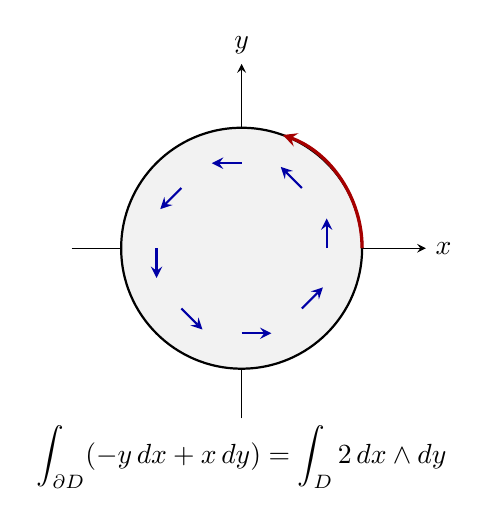
\begin{tikzpicture}[scale=0.9, >=stealth]
    \draw[->] (-2.4,0) -- (2.6,0) node[right] {\(x\)};
    \draw[->] (0,-2.4) -- (0,2.6) node[above] {\(y\)};

    \draw[fill=gray!10, thick] (0,0) circle (1.7);

    \draw[->, very thick, red!65!black]
        (1.7,0) arc[start angle=0,end angle=70,radius=1.7];

    \foreach \x/\y in {
        1.2/0,0.85/0.85,0/1.2,-0.85/0.85,-1.2/0,
        -0.85/-0.85,0/-1.2,0.85/-0.85
    } {
        \draw[->, blue!65!black, thick]
            (\x,\y) -- ++({-0.35*\y},{0.35*\x});
    }

    \node at (0,-2.95)
        {\(\displaystyle \int_{\partial D}(-y\,dx+x\,dy)=\int_D2\,dx\wedge dy\)};
\end{tikzpicture}
\caption{The boundary integral measures circulation.  The exterior derivative measures
circulation per unit area.}
\end{figure}

\subsubsection*{Your task}

Choose one classical vector calculus problem and translate it completely into forms.

Use one of the following, or choose your own.

\[
\begin{array}{c|c|c}
\text{Classical problem} & \text{Classical theorem} & \text{Forms version} \\ \hline
\oint_C \mathbf F\cdot d\mathbf r
&
\text{Green's theorem}
&
\int_{\partial R}\omega=\int_R d\omega
\\[1mm]
\oint_{\partial S}\mathbf F\cdot d\mathbf r
&
\text{Stokes' theorem}
&
\int_{\partial S}\omega=\int_S d\omega
\\[1mm]
\iint_{\partial E}\mathbf F\cdot\widehat{\mathbf n}\,dS
&
\text{Divergence theorem}
&
\int_{\partial E}\Phi=\int_E d\Phi
\\[1mm]
\int_C \nabla f\cdot d\mathbf r
&
\text{Fundamental theorem for line integrals}
&
\int_C df=\int_{\partial C}f
\end{array}
\]

\subsubsection*{Suggested examples}

\[
\begin{array}{c|c}
\text{Example} & \text{What to translate} \\ \hline
\mathbf F=(-y/2,x/2) \text{ around an ellipse}
&
\text{area from circulation}\\[1mm]
\mathbf F=(x,y,z) \text{ through a box}
&
\text{flux and divergence}\\[1mm]
\mathbf F=(-y,x,0) \text{ around a disk in space}
&
\text{Stokes' theorem}\\[1mm]
f(x,y,z)=x^2y+z
&
\text{gradient field and }df
\end{array}
\]

\subsubsection*{Required steps}

\begin{enumerate}
\item State the classical problem.

\item Identify the correct form:
\[
    \omega=P\,dx+Q\,dy+R\,dz
\]
or
\[
    \Phi=P\,dy\wedge dz+Q\,dz\wedge dx+R\,dx\wedge dy.
\]

\item Compute the exterior derivative:
\[
    d\omega
    \qquad\text{or}\qquad
    d\Phi.
\]

\item Compute the integral directly, if possible.

\item Compute the integral using
\[
    \int_{\partial M}\omega=\int_Md\omega.
\]

\item Write a translation table showing each classical object and its forms version.

\item Explain which notation made orientation easier to track.
\end{enumerate}

\subsubsection*{What to hand in}

Your report should include:

\begin{enumerate}
\item the original classical problem,

\item the form version of the problem,

\item the calculation of \(d\omega\) or \(d\Phi\),

\item both sides of the theorem,

\item a short translation table,

\item a paragraph explaining what the forms notation clarifies.
\end{enumerate}

The best reports do not merely replace dots and crosses by wedges.  They explain why
the form is the natural integrand for the geometric object.

\subsection{Project 2: closed but not exact forms on punctured domains}

A \(1\)-form \(\omega\) is called \emph{closed} if
\[
    d\omega=0.
\]
It is called \emph{exact} if there is a function \(f\) such that
\[
    \omega=df.
\]
Every exact form is closed, because
\[
    d(df)=0.
\]
But the converse can fail when the domain has a hole.

This project is about that failure.

\subsubsection*{A seed example: the angular form}

On the punctured plane
\[
    \mathbb R^2\setminus\{(0,0)\},
\]
define
\[
\boxed{
    \omega=
    \frac{-y\,dx+x\,dy}{x^2+y^2}.
}
\]
This form measures change in angle around the origin.

Let
\[
    P=\frac{-y}{x^2+y^2},
    \qquad
    Q=\frac{x}{x^2+y^2}.
\]
Then
\[
    \omega=P\,dx+Q\,dy.
\]
Compute:
\[
\begin{aligned}
    Q_x
    &=
    \frac{(x^2+y^2)-2x^2}{(x^2+y^2)^2}
    =
    \frac{y^2-x^2}{(x^2+y^2)^2},
\end{aligned}
\]
and
\[
\begin{aligned}
    P_y
    &=
    \frac{-(x^2+y^2)+2y^2}{(x^2+y^2)^2}
    =
    \frac{y^2-x^2}{(x^2+y^2)^2}.
\end{aligned}
\]
Thus
\[
    Q_x-P_y=0.
\]
So
\[
\boxed{
    d\omega=0.
}
\]
The form is closed.

Now integrate around the unit circle:
\[
    x=\cos t,\qquad y=\sin t,\qquad 0\le t\le2\pi.
\]
Then
\[
    dx=-\sin t\,dt,
    \qquad
    dy=\cos t\,dt,
\]
and
\[
    x^2+y^2=1.
\]
Therefore
\[
\begin{aligned}
    \omega
    &=
    -\sin t(-\sin t\,dt)+\cos t(\cos t\,dt)\\
    &=
    dt.
\end{aligned}
\]
So
\[
\boxed{
    \oint_C\omega=2\pi.
}
\]

If \(\omega\) were exact on the punctured plane, say
\[
    \omega=df,
\]
then every closed-curve integral would be zero:
\[
    \oint_C df=f(\text{endpoint})-f(\text{starting point})=0.
\]
But we found
\[
    \oint_C\omega=2\pi.
\]
So \(\omega\) is closed but not exact on
\[
    \mathbb R^2\setminus\{(0,0)\}.
\]

The missing origin stores the obstruction.

\begin{figure}[h]
\centering
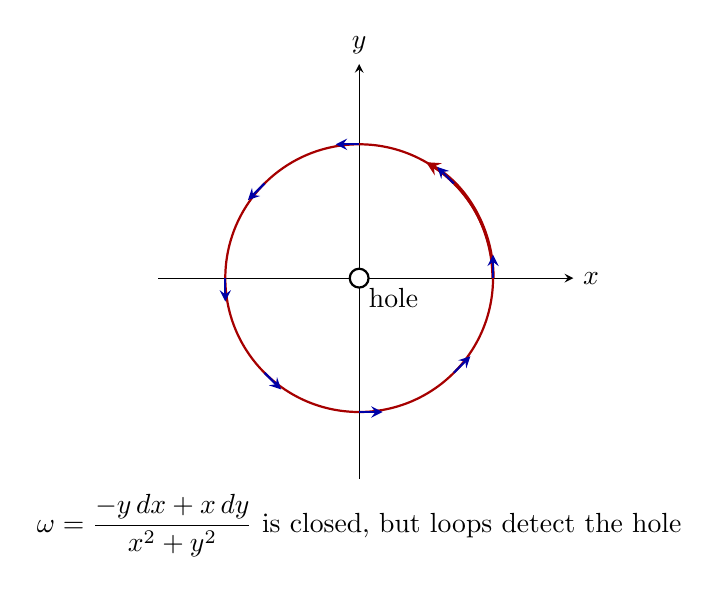
\begin{tikzpicture}[scale=0.85, >=stealth]
    \draw[->] (-3,0) -- (3.2,0) node[right] {\(x\)};
    \draw[->] (0,-3) -- (0,3.2) node[above] {\(y\)};

    \fill[white] (0,0) circle (4pt);
    \draw[thick] (0,0) circle (4pt);
    \node[below right] at (0,0) {hole};

    \draw[thick, red!65!black] (0,0) circle (2);
    \draw[->, very thick, red!65!black]
        (2,0) arc[start angle=0,end angle=60,radius=2];

    \foreach \ang in {0,45,90,135,180,225,270,315} {
        \pgfmathsetmacro{\x}{2*cos(\ang)}
        \pgfmathsetmacro{\y}{2*sin(\ang)}
        \draw[->, blue!65!black, thick]
            (\x,\y) -- ++({-0.35*sin(\ang)},{0.35*cos(\ang)});
    }

    \node at (0,-3.7)
        {\(\displaystyle \omega=\frac{-y\,dx+x\,dy}{x^2+y^2}\) is closed, but loops detect the hole};
\end{tikzpicture}
\caption{A closed form can fail to be exact when the domain has a hole.}
\end{figure}

\subsubsection*{Your task}

Study one closed form on a punctured domain.

Use one of the following.

\[
\begin{array}{c|c}
\text{Form} & \text{Domain} \\ \hline
\displaystyle
\omega_1=\frac{-y\,dx+x\,dy}{x^2+y^2}
&
\mathbb R^2\setminus\{(0,0)\}
\\[4mm]
\displaystyle
\omega_2=\frac{x\,dx+y\,dy}{x^2+y^2}
&
\mathbb R^2\setminus\{(0,0)\}
\\[4mm]
\displaystyle
\omega_3=
\frac{-(y-b)\,dx+(x-a)\,dy}{(x-a)^2+(y-b)^2}
&
\mathbb R^2\setminus\{(a,b)\}
\end{array}
\]

The second form is different from the angular form.  In fact,
\[
    \omega_2=d\left(\ln\sqrt{x^2+y^2}\right).
\]
So \(\omega_2\) is exact on the punctured plane.  Comparing \(\omega_1\) and
\(\omega_2\) is a good way to see that ``closed'' and ``exact'' are not the same idea.

\subsubsection*{Required steps}

\begin{enumerate}
\item State the domain carefully.  Do not include points where the formula is undefined.

\item Compute \(d\omega\).

\item Decide whether the form is closed.

\item Integrate \(\omega\) around at least two closed curves:
\[
    \text{one loop that surrounds the missing point}
\]
and
\[
    \text{one loop that does not surround the missing point}.
\]

\item Decide whether the form is exact on the whole domain.

\item If possible, find a potential function on a smaller domain, such as a plane with a
ray removed.

\item Explain what the hole changes.
\end{enumerate}

\subsubsection*{Questions to answer}

\begin{enumerate}
\item Why does \(d\omega=0\) not automatically imply \(\omega=df\)?

\item What happens to the integral if a loop winds around the puncture twice?

\item Why does a loop that does not surround the puncture give a different kind of
answer?

\item What is the role of the angle function \(\theta\)?  Why can it be chosen locally but
not globally around the puncture?

\item What does this example teach about the hypotheses in conservative-field
theorems?
\end{enumerate}

\subsubsection*{What to hand in}

Your report should include:

\begin{enumerate}
\item the form and its domain,

\item the calculation of \(d\omega\),

\item at least two closed-curve integrals,

\item a conclusion about closedness and exactness,

\item a drawing of the domain and the loops,

\item a paragraph explaining why the missing point matters.
\end{enumerate}

The important lesson is not the formula itself.  The important lesson is that local
information can miss global topology.  A form may have no local curl and still remember
a hole.

\subsection{Project 3: the generalized Stokes theorem on a cube}

The generalized Stokes theorem says
\[
\boxed{
    \int_{\partial M}\omega=\int_M d\omega.
}
\]
For a solid cube, the form \(\omega\) must be a \(2\)-form, because the boundary of a
solid is a surface.

This project asks you to verify the theorem face by face.

\subsubsection*{A seed example: a flux form on the unit cube}

Let
\[
    B=[0,1]\times[0,1]\times[0,1]
\]
with orientation
\[
    dx\wedge dy\wedge dz.
\]
Consider the \(2\)-form
\[
\boxed{
    \Phi
    =
    x\,dy\wedge dz
    +
    y\,dz\wedge dx
    +
    z\,dx\wedge dy.
}
\]
This is the flux form of the vector field
\[
    \mathbf F=(x,y,z).
\]

First compute the exterior derivative:
\[
\begin{aligned}
d\Phi
&=
d(x\,dy\wedge dz)
+
d(y\,dz\wedge dx)
+
d(z\,dx\wedge dy)\\
&=
dx\wedge dy\wedge dz
+
dy\wedge dz\wedge dx
+
dz\wedge dx\wedge dy.
\end{aligned}
\]
Both
\[
    dy\wedge dz\wedge dx
\]
and
\[
    dz\wedge dx\wedge dy
\]
are cyclic rearrangements of
\[
    dx\wedge dy\wedge dz,
\]
so they have the same sign.  Thus
\[
\boxed{
    d\Phi=3\,dx\wedge dy\wedge dz.
}
\]
Therefore
\[
\boxed{
    \int_B d\Phi=3.
}
\]

Now compute the boundary integral.  The boundary has six faces.

Using the outward orientation, the induced face orientations are:

\[
\begin{array}{c|c}
\text{Face} & \text{Induced orientation} \\ \hline
x=1 & dy\wedge dz\\
x=0 & -dy\wedge dz\\
y=1 & dz\wedge dx\\
y=0 & -dz\wedge dx\\
z=1 & dx\wedge dy\\
z=0 & -dx\wedge dy
\end{array}
\]

On the face \(x=1\),
\[
    \Phi=1\,dy\wedge dz+\text{terms involving }dx.
\]
Terms involving \(dx\) vanish on this face because \(x\) is constant there.  Hence
\[
    \int_{x=1}\Phi=1.
\]

On the face \(x=0\), the coefficient \(x\) is zero, so the contribution is
\[
    0.
\]

Similarly,
\[
    \int_{y=1}\Phi=1,
    \qquad
    \int_{y=0}\Phi=0,
\]
and
\[
    \int_{z=1}\Phi=1,
    \qquad
    \int_{z=0}\Phi=0.
\]

Thus
\[
\boxed{
    \int_{\partial B}\Phi=1+1+1=3.
}
\]
So
\[
\boxed{
    \int_{\partial B}\Phi=\int_B d\Phi.
}
\]


\subsubsection*{Your task}

Verify the generalized Stokes theorem on a rectangular box or cube.

Choose one of these.

\[
\begin{array}{c|c}
\text{Region} & \text{Form} \\ \hline
[0,1]^3 &
x\,dy\wedge dz+y\,dz\wedge dx+z\,dx\wedge dy\\[1mm]
[0,a]\times[0,b]\times[0,c] &
x^2\,dy\wedge dz+y\,dz\wedge dx+z\,dx\wedge dy\\[1mm]
[0,1]^2 &
(x^2+y)\,dx+xy\,dy\\[1mm]
[0,a]\times[0,b] &
-y\,dx+x\,dy
\end{array}
\]

The three-dimensional choices verify the divergence theorem in forms language.  The
two-dimensional choices verify Green's theorem in forms language.

\subsubsection*{Required steps}

\begin{enumerate}
\item State the region and its orientation.

\item State the form \(\omega\).

\item Compute \(d\omega\).

\item Compute the interior integral:
\[
    \int_M d\omega.
\]

\item List all boundary pieces.

\item State the induced orientation on each boundary piece.

\item Compute each boundary contribution.

\item Add the boundary contributions and compare with the interior integral.
\end{enumerate}

\subsubsection*{Questions to answer}

\begin{enumerate}
\item Which boundary pieces contribute zero?  Why?

\item Where does orientation enter the calculation?

\item What would change if the region were given the opposite orientation?

\item In the three-dimensional case, what vector field has the chosen \(2\)-form as its
flux form?

\item In the two-dimensional case, what vector field has the chosen \(1\)-form as its
work form?
\end{enumerate}

\subsubsection*{What to hand in}

Your report should include:

\begin{enumerate}
\item a drawing of the region,

\item the form and its exterior derivative,

\item the interior integral,

\item a table of boundary pieces and orientations,

\item the boundary integral,

\item a sentence explaining how this example fits
\[
    \int_{\partial M}\omega=\int_Md\omega.
\]
\end{enumerate}

A cube is simple enough that no geometry is hidden.  Every sign must be earned.  That is
why it is such a good testing ground for Stokes' theorem.

\subsection{Project 4: orientation errors as sign errors}

Many wrong answers in vector calculus are not calculus mistakes.  They are orientation
mistakes.

A curve is walked the wrong way.  A normal vector points inward instead of outward.
An inner boundary is treated like an outer boundary.  A parametrization reverses the
surface orientation.

Forms do not remove these errors, but they make them visible.  A form changes sign
when orientation reverses.  If the sign is wrong, the geometry is usually wrong too.

\subsubsection*{A seed example: the annulus and the inner boundary}

Let \(A\) be the annulus
\[
    1\le x^2+y^2\le4.
\]
Consider the \(1\)-form
\[
\boxed{
    \eta=\frac12(x\,dy-y\,dx).
}
\]
Then
\[
\begin{aligned}
d\eta
&=
\frac12(dx\wedge dy-dy\wedge dx)\\
&=
dx\wedge dy.
\end{aligned}
\]
So Green's theorem says
\[
\boxed{
    \int_{\partial A}\eta
    =
    \int_A dx\wedge dy
    =
    \operatorname{Area}(A).
}
\]

The area is
\[
    \pi(2^2)-\pi(1^2)=3\pi.
\]

Now compute the boundary integral.  On a counterclockwise circle of radius \(R\),
\[
    x=R\cos t,\qquad y=R\sin t.
\]
Then
\[
    dx=-R\sin t\,dt,
    \qquad
    dy=R\cos t\,dt,
\]
so
\[
\begin{aligned}
    \eta
    &=
    \frac12
    \left(
        R\cos t(R\cos t\,dt)
        -
        R\sin t(-R\sin t\,dt)
    \right)\\
    &=
    \frac12R^2\,dt.
\end{aligned}
\]
Therefore
\[
    \int_{\text{ccw circle radius }R}\eta
    =
    \pi R^2.
\]

The outer boundary of the annulus is oriented counterclockwise, so it contributes
\[
    4\pi.
\]
The inner boundary is oriented clockwise, so it contributes
\[
    -\pi.
\]
Thus
\[
\boxed{
    \int_{\partial A}\eta=4\pi-\pi=3\pi.
}
\]

If we accidentally orient the inner boundary counterclockwise, we get
\[
    4\pi+\pi=5\pi.
\]
That answer is not the area of the annulus.  The sign error has added the hole instead
of subtracting it.

\begin{figure}[h]
\centering
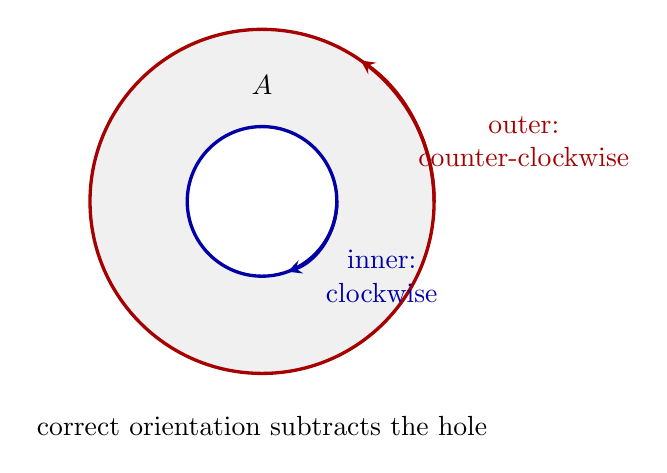
\begin{tikzpicture}[scale=0.95, >=stealth]
    \draw[fill=gray!12, even odd rule]
        (0,0) circle (2.3)
        (0,0) circle (1.0);

    \draw[very thick, red!65!black] (0,0) circle (2.3);
    \draw[->, very thick, red!65!black]
        (2.3,0) arc[start angle=0,end angle=55,radius=2.3];

    \draw[very thick, blue!65!black] (0,0) circle (1.0);
    \draw[->, very thick, blue!65!black]
        (1,0) arc[start angle=0,end angle=-70,radius=1.0];

    \node at (0,1.55) {\(A\)};
    \node[red!65!black, align=center] at (3.5,0.8) {outer:\\counter-clockwise};
    \node[blue!65!black, align=center] at (1.6,-1.0) {inner:\\clockwise};

    \node at (0,-3.0) {correct orientation subtracts the hole};
\end{tikzpicture}
\caption{An inner boundary is positively oriented clockwise, because the region must
stay on the left.}
\end{figure}

\subsubsection*{Your task}

Choose one orientation-sensitive problem and compute it twice: once correctly and once
with a common orientation error.

Use one of these.

\[
\begin{array}{c|c}
\text{Problem} & \text{Common sign error} \\ \hline
\text{annulus area from } \eta=\frac12(x\,dy-y\,dx)
&
\text{inner boundary walked counterclockwise}\\[1mm]
\text{flux through a closed box}
&
\text{one face normal points inward}\\[1mm]
\text{Stokes' theorem on a disk}
&
\text{boundary direction disagrees with normal}\\[1mm]
\text{surface integral over a parametrized surface}
&
\text{parameters swapped}\\[1mm]
\text{Green's theorem on a rectangle}
&
\text{boundary walked clockwise}
\end{array}
\]

\subsubsection*{Required steps}

\begin{enumerate}
\item State the region, curve, or surface.

\item State its correct orientation.

\item Compute the integral correctly.

\item Deliberately make one orientation error.

\item Compute the incorrect result.

\item Explain exactly where the sign changed.

\item State a practical rule for avoiding that error.
\end{enumerate}

\subsubsection*{Orientation checklist}

Use this checklist in your report.

\[
\begin{array}{c|l}
\text{Object} & \text{Positive orientation rule} \\ \hline
\text{interval} & \text{right endpoint positive, left endpoint negative}\\[1mm]
\text{plane region} & \text{walk so the region stays on the left}\\[1mm]
\text{surface in space} & \text{right-hand rule connects normal and boundary}\\[1mm]
\text{solid} & \text{boundary surface points outward}\\[1mm]
\text{parametrized surface} & \mathbf r_u\times\mathbf r_v \text{ gives the chosen normal}
\end{array}
\]

\subsubsection*{What to hand in}

Your report should include:

\begin{enumerate}
\item a drawing showing the correct orientation,

\item the correct calculation,

\item the incorrect calculation,

\item a comparison of the two answers,

\item a short ``sign diagnosis'' explaining the mistake,

\item a final checklist for future problems.
\end{enumerate}

These forms projects are computational, but they also train a habit of attention:
integrals do not live on shapes alone.  They live on oriented shapes.  The last projects
in the chapter ask for a different skill.  After learning to compute, translate, and check
signs, a mathematician has one more job: explain the story clearly enough that someone
else can see why it matters.

\section{Writing projects}
\label{sec:20.6}

A calculation can be correct and still leave the reader unmoved.  A good mathematical
essay does more.  It chooses a question, follows it honestly, explains the necessary
ideas, and ends with a sharper understanding than it began with.

These writing projects are not research papers in the graduate-school sense.  They are
mathematical explanations.  The goal is to take one thread from the book and tell its
story.

A good essay should contain:

\[
\begin{array}{ll}
1. & \text{a clear central question,}\\
2. & \text{at least two worked mathematical examples,}\\
3. & \text{a diagram, table, or carefully described picture,}\\
4. & \text{a connection to earlier chapters,}\\
5. & \text{a conclusion that says what changed in your understanding.}
\end{array}
\]

\subsection{Project 1: Hamilton, quaternions, and the birth of vector algebra}

Chapter \ref{ch:2} began with a strange question:

\[
    \text{Can we multiply vectors?}
\]

In the plane, complex numbers answered yes.  Multiplication by
\[
    a+bi
\]
rotates and stretches.  But in three dimensions, the answer was harder.  Hamilton's
quaternions gave one answer, and modern vector algebra later split that answer into
the dot product and cross product.

This writing project asks you to explain that split.

\subsubsection*{A seed calculation}

A pure imaginary quaternion has the form
\[
    A=a_1i+a_2j+a_3k.
\]
We identify it with the vector
\[
    \mathbf a=(a_1,a_2,a_3).
\]
Similarly,
\[
    B=b_1i+b_2j+b_3k
\]
corresponds to
\[
    \mathbf b=(b_1,b_2,b_3).
\]

Using
\[
    i^2=j^2=k^2=-1,
\]
and
\[
    ij=k,\qquad jk=i,\qquad ki=j,
\]
with the reversed products changing sign, one finds
\[
\boxed{
    AB=-\mathbf a\cdot\mathbf b+\mathbf a\times\mathbf b.
}
\]
More explicitly,
\[
\begin{aligned}
AB
&=
-(a_1b_1+a_2b_2+a_3b_3)\\
&\qquad
+
(a_2b_3-a_3b_2)i\\
&\qquad
+
(a_3b_1-a_1b_3)j\\
&\qquad
+
(a_1b_2-a_2b_1)k.
\end{aligned}
\]
The scalar part is
\[
    -\mathbf a\cdot\mathbf b.
\]
The vector part is
\[
    \mathbf a\times\mathbf b.
\]

So the dot product and cross product were not born as two unrelated formulas.  They
are two pieces of one multiplication.

\subsubsection*{Your task}

Write an essay explaining how quaternions connect complex numbers, dot products, and
cross products.

Your essay should answer:

\begin{enumerate}
\item Why does complex multiplication feel geometrically natural in the plane?

\item What changes when we try to multiply triples?

\item What are the rules for quaternion units \(i,j,k\)?

\item Why is quaternion multiplication noncommutative?

\item How do the dot product and cross product appear inside the product of two pure
imaginary quaternions?

\item Why did vector algebra eventually separate the scalar part and vector part?

\item How does the wedge product give another way to think about oriented area?
\end{enumerate}

\subsubsection*{Required mathematical examples}

Include at least two of the following:

\[
\begin{array}{c|c}
\text{Example} & \text{Purpose} \\ \hline
(1+i)(1-i)=2 & \text{complex multiplication and length}\\[1mm]
ij=k,\quad ji=-k & \text{noncommutativity}\\[1mm]
(i+j)(i-j) & \text{scalar and vector parts}\\[1mm]
(1,0,0)\times(0,1,0)=(0,0,1)
& \text{cross product orientation}\\[1mm]
\mathbf a\wedge\mathbf b
& \text{oriented area without choosing a normal vector}
\end{array}
\]

\subsubsection*{What to hand in}

Submit a \(3\)- to \(5\)-page essay with:

\begin{enumerate}
\item a title,

\item a clear thesis statement,

\item at least two worked examples,

\item one diagram,

\item a short comparison between quaternions and the vector operations used in this
book,

\item a bibliography or source list if historical claims are included.
\end{enumerate}

A strong essay will not only say that quaternions came before vector algebra.  It will
show, through a calculation, why dot and cross products are two shadows of a larger
multiplication.

\subsection{Project 2: why the cross product is both useful and suspicious}

The cross product is one of the most useful tools in three-dimensional calculus:
\[
    \mathbf u\times\mathbf v.
\]
It gives normal vectors, areas of parallelograms, torque, angular momentum, and the
curl of a vector field.

But it is also suspicious.

Two vectors in the plane span an oriented parallelogram.  Two vectors in space also
span an oriented parallelogram.  The cross product replaces that parallelogram by a
perpendicular vector.  This works beautifully in \(\mathbb R^3\), because a plane has one
perpendicular direction, up to sign.

But the geometric object created by two vectors is really an oriented area element, not
a vector.  The wedge product keeps it as an oriented area:
\[
    \mathbf u\wedge\mathbf v.
\]
The cross product turns it into a vector by using extra structure: distance, angle, and
orientation of space.

\subsubsection*{A seed comparison}

Let
\[
    \mathbf u=(1,0,0),
    \qquad
    \mathbf v=(0,2,0).
\]
The parallelogram has area
\[
    2.
\]
The cross product is
\[
    \mathbf u\times\mathbf v=(0,0,2).
\]
This vector has length \(2\) and points in the positive \(z\)-direction.

The wedge product instead records
\[
    \mathbf u\wedge\mathbf v=2\,dx\wedge dy.
\]
It says: the oriented area lies in the \(xy\)-direction and has signed size \(2\).

Both descriptions contain the same area information in three dimensions.  But they
store it differently.

\subsubsection*{Your task}

Write an essay explaining the double personality of the cross product.

Your essay should argue both sides:

\[
\begin{array}{c|l}
\text{Useful} & \text{The cross product gives quick normal vectors and area vectors.}\\[1mm]
\text{Suspicious} & \text{It turns an oriented area into a vector using special features of } \mathbb R^3.
\end{array}
\]

\subsubsection*{Questions to answer}

\begin{enumerate}
\item What geometric quantity is \(\|\mathbf u\times\mathbf v\|\) measuring?

\item Why does the direction of \(\mathbf u\times\mathbf v\) depend on orientation?

\item Why does swapping the vectors change the sign?
\[
    \mathbf v\times\mathbf u=-(\mathbf u\times\mathbf v).
\]

\item Why is a surface area element more naturally written as
\[
    dx\wedge dy,\qquad dy\wedge dz,\qquad dz\wedge dx
\]
than as a normal vector?

\item Why is the cross product especially convenient for parametrized surfaces?

\item What does forms language clarify about flux?
\end{enumerate}

\subsubsection*{Required examples}

Include at least three examples:

\[
\begin{array}{c|c}
\text{Example} & \text{Concept} \\ \hline
\mathbf r_u\times\mathbf r_v & \text{surface normal and area scale}\\[1mm]
\mathbf r_v\times\mathbf r_u & \text{orientation reversal}\\[1mm]
\mathbf F\cdot(\mathbf r_u\times\mathbf r_v)\,du\,dv
&
\text{classical flux}\\[1mm]
\Phi_{\mathbf F}=
F_1\,dy\wedge dz+F_2\,dz\wedge dx+F_3\,dx\wedge dy
&
\text{forms flux}\\[1mm]
\mathbf u\wedge\mathbf v
&
\text{oriented area before choosing a normal}
\end{array}
\]

\subsubsection*{What to hand in}

Submit a \(3\)- to \(5\)-page essay with:

\begin{enumerate}
\item a clear thesis,

\item a diagram of an oriented parallelogram,

\item at least three worked examples,

\item one paragraph defending the cross product,

\item one paragraph criticizing or limiting the cross product,

\item a concluding paragraph explaining what the wedge product changes.
\end{enumerate}

The best essays will not treat the cross product as wrong.  It is not wrong.  It is a
brilliant shortcut.  But every shortcut hides a path, and forms reveal the path.

\subsection{Project 3: the many lives of the Fundamental Theorem of Calculus}

Single-variable calculus has a central theorem:
\[
\boxed{
    \int_a^b f'(x)\,dx=f(b)-f(a).
}
\]
This theorem says that adding derivative information over an interval gives boundary
information at the endpoints.

By the end of this book, the same sentence has grown into
\[
\boxed{
    \int_{\partial M}\omega=\int_Md\omega.
}
\]

This writing project asks you to tell that story.

\subsubsection*{A seed table}

\[
\begin{array}{c|c|c}
\text{Object }M & \text{Form }\omega & \text{Theorem} \\ \hline
[a,b] & f &
\displaystyle
\int_{\partial[a,b]}f=\int_{[a,b]}df
\\[3mm]
\text{plane region }R & P\,dx+Q\,dy &
\displaystyle
\int_{\partial R}\omega=\int_Rd\omega
\\[3mm]
\text{surface }S & P\,dx+Q\,dy+R\,dz &
\displaystyle
\int_{\partial S}\omega=\int_Sd\omega
\\[3mm]
\text{solid }E &
P\,dy\wedge dz+Q\,dz\wedge dx+R\,dx\wedge dy
&
\displaystyle
\int_{\partial E}\Phi=\int_Ed\Phi
\end{array}
\]

In the first row,
\[
    \partial[a,b]=\{b\}-\{a\},
\]
so
\[
    \int_{\partial[a,b]}f=f(b)-f(a).
\]

In the last row,
\[
    d\Phi=(P_x+Q_y+R_z)\,dx\wedge dy\wedge dz,
\]
so the theorem becomes the divergence theorem.

The boundary changes dimension.  The form changes degree.  But the pattern does not
change.

\subsubsection*{Your task}

Write an essay explaining how the Fundamental Theorem of Calculus reappears as:

\[
\begin{array}{ll}
1. & \text{the Fundamental Theorem for line integrals,}\\
2. & \text{Green's theorem,}\\
3. & \text{Stokes' theorem,}\\
4. & \text{the divergence theorem,}\\
5. & \text{the generalized Stokes theorem.}
\end{array}
\]

You do not need to prove every theorem.  Your job is to explain the shared structure.

\subsubsection*{Required examples}

Include at least three worked examples, chosen from different dimensions.

\[
\begin{array}{c|c}
\text{Example} & \text{Boundary principle} \\ \hline
\displaystyle \int_1^4 d(x^2+1)
&
\text{endpoints}\\[2mm]
\displaystyle \int_C df
&
\text{potential difference}\\[2mm]
\displaystyle \int_{\partial R}x\,dy
&
\text{area from boundary}\\[2mm]
\displaystyle \int_{\partial B}
\left(x\,dy\wedge dz+y\,dz\wedge dx+z\,dx\wedge dy\right)
&
\text{flux from divergence}\\[3mm]
\displaystyle \int_{\partial S}\omega
&
\text{circulation from surface curl}
\end{array}
\]

\subsubsection*{Questions to answer}

\begin{enumerate}
\item What does ``boundary'' mean for an interval, a region, a surface, and a solid?

\item Why do signs and orientations become unavoidable?

\item What changes when \(d\) acts on a \(0\)-form, a \(1\)-form, and a \(2\)-form?

\item How do gradient, curl, and divergence fit into one operation?

\item Why is the statement
\[
    \int_{\partial M}\omega=\int_Md\omega
\]
not just shorter, but more revealing?
\end{enumerate}

\subsubsection*{What to hand in}

Submit a \(4\)- to \(6\)-page essay with:

\begin{enumerate}
\item a central thesis,

\item a translation table,

\item at least three examples,

\item at least one diagram showing an object and its boundary,

\item a paragraph on orientation,

\item a conclusion explaining what the word ``fundamental'' means after this course.
\end{enumerate}

A strong essay should make the reader feel that the Fundamental Theorem did not
disappear after single-variable calculus.  It kept changing clothes.

\subsection{Project 4: how conservation laws unify physics and calculus}

Chapter \ref{ch:19} added time to Stokes' theorem.  A conserved quantity can be stored
inside a region, carried across the boundary, and created or destroyed by sources.

That gives the bookkeeping law
\[
\boxed{
    \frac{d}{dt}\iiint_E \rho\,dV
    +
    \iint_{\partial E}\mathbf J\cdot\widehat{\mathbf n}\,dS
    =
    \iiint_E s\,dV.
}
\]
Here:

\[
\begin{array}{c|c}
\rho & \text{density stored inside the region}\\[1mm]
\mathbf J & \text{flux density crossing the boundary}\\[1mm]
s & \text{source rate per unit volume}
\end{array}
\]

In forms language, the flux term becomes
\[
    \int_{\partial E}\Phi_{\mathbf J},
\]
where
\[
    \Phi_{\mathbf J}
    =
    J_1\,dy\wedge dz
    +
    J_2\,dz\wedge dx
    +
    J_3\,dx\wedge dy.
\]
By Stokes' theorem,
\[
    \int_{\partial E}\Phi_{\mathbf J}
    =
    \int_E d\Phi_{\mathbf J}.
\]
Since
\[
    d\Phi_{\mathbf J}
    =
    (\nabla\cdot\mathbf J)\,dx\wedge dy\wedge dz,
\]
the integral balance becomes, locally,
\[
\boxed{
    \rho_t+\nabla\cdot\mathbf J=s.
}
\]

That equation is the skeleton of many physical theories.

\subsubsection*{A seed explanation: dye in water}

Let \(\rho\) be dye density and let \(\mathbf J=\rho\mathbf v\) be dye flux density.
If there are no sources, then
\[
    s=0.
\]
The local conservation law becomes
\[
\boxed{
    \rho_t+\nabla\cdot(\rho\mathbf v)=0.
}
\]
This says:

\[
\text{rate of change of stored dye}
+
\text{net outward flow of dye}
=
0.
\]

If more dye flows out of a small region than flows in, the density inside must decrease.
If more flows in than out, the density must increase.

The equation is not a mysterious new law.  It is careful accounting.

\subsubsection*{Your task}

Write an essay explaining how conservation laws connect calculus to physics.

Choose one theme:

\[
\begin{array}{c|c}
\text{Theme} & \text{Possible law} \\ \hline
\text{fluid or dye flow} & \rho_t+\nabla\cdot(\rho\mathbf v)=0\\[1mm]
\text{heat flow} & u_t=\kappa\Delta u\\[1mm]
\text{electric charge} & \rho_t+\nabla\cdot\mathbf J=0\\[1mm]
\text{population movement} & \rho_t+\nabla\cdot(\rho\mathbf v)=s\\[1mm]
\text{chemical concentration} & \rho_t+\nabla\cdot\mathbf J=s
\end{array}
\]

\subsubsection*{Required structure}

Your essay should include:

\begin{enumerate}
\item A physical story.  What is moving, stored, created, or destroyed?

\item A density \(\rho\).  What does it measure?

\item A flux \(\mathbf J\).  What does it mean physically?

\item A source term \(s\), or a clear statement that \(s=0\).

\item The integral balance law over a fixed region \(E\).

\item The local differential equation.

\item An explanation of how the divergence theorem or Stokes' theorem connects the
two.
\end{enumerate}

\subsubsection*{A useful derivation to include}

Start with
\[
    \frac{d}{dt}\iiint_E \rho\,dV
    +
    \iint_{\partial E}\mathbf J\cdot\widehat{\mathbf n}\,dS
    =
    \iiint_E s\,dV.
\]
Use the divergence theorem:
\[
    \iint_{\partial E}\mathbf J\cdot\widehat{\mathbf n}\,dS
    =
    \iiint_E\nabla\cdot\mathbf J\,dV.
\]
Then
\[
    \iiint_E \rho_t\,dV
    +
    \iiint_E\nabla\cdot\mathbf J\,dV
    =
    \iiint_E s\,dV.
\]
So
\[
    \iiint_E
    \left(
        \rho_t+\nabla\cdot\mathbf J-s
    \right)dV=0.
\]
If this holds for every reasonable fixed region \(E\), then the integrand must vanish:
\[
\boxed{
    \rho_t+\nabla\cdot\mathbf J=s.
}
\]

In forms notation, the same derivation is
\[
    \frac{d}{dt}\int_E \rho\,dx\wedge dy\wedge dz
    +
    \int_{\partial E}\Phi_{\mathbf J}
    =
    \int_E s\,dx\wedge dy\wedge dz,
\]
then
\[
    \int_E
    \left(
        \rho_t\,dx\wedge dy\wedge dz
        +
        d\Phi_{\mathbf J}
        -
        s\,dx\wedge dy\wedge dz
    \right)=0.
\]

\subsubsection*{Questions to answer}

\begin{enumerate}
\item What does outward flux mean in your physical setting?

\item Why does outward flux appear with a plus sign in the balance equation but causes
stored amount to decrease when there are no sources?

\item What does a positive source term mean?

\item What does the local equation say in ordinary language?

\item Where does Stokes' theorem enter?

\item Why do very different systems share the same mathematical form?
\end{enumerate}

\subsubsection*{What to hand in}

Submit a \(4\)- to \(6\)-page essay with:

\begin{enumerate}
\item a physical introduction,

\item the integral balance law,

\item the local differential equation,

\item at least one worked example with simple functions,

\item a diagram of a region with flux arrows crossing its boundary,

\item a paragraph connecting the derivation to the generalized Stokes theorem.
\end{enumerate}

\subsection*{A short rubric for the writing projects}

\[
\begin{array}{c|p{9cm}}
\text{Criterion} & \text{What a strong submission does} \\ \hline
\text{Thesis} & States a clear mathematical question or claim.\\[1mm]
\text{Examples} & Uses concrete computations, not only general statements.\\[1mm]
\text{Accuracy} & Keeps definitions, signs, and notation correct.\\[1mm]
\text{Connection} & Links the topic to earlier chapters of the book.\\[1mm]
\text{Clarity} & Explains ideas in complete sentences, with diagrams or tables where helpful.\\[1mm]
\text{Reflection} & Ends by saying what the project reveals that a formula alone would hide.
\end{array}
\]

This chapter began as a workshop, but it ends as a mirror for the whole book.  Vectors
gave us direction.  Derivatives gave us local change.  Integrals gave us accumulation.
Forms gave us the right integrands for curves, surfaces, and solids.  Stokes' theorem
tied boundaries to interiors.

The story is not finished.  It never is.  But the next time a problem asks you to measure
change, flow, circulation, flux, or balance, you have a question that reaches farther than
any single formula:

\[
\boxed{
    \text{What is the object, what is its boundary, and what form belongs on it?}
}
\]
